%-----------------------------------------------------------------------------
%
%               Template for sigplanconf LaTeX Class
%
% Name:         sigplanconf-template.tex
%
% Purpose:      A template for sigplanconf.cls, which is a LaTeX 2e class
%               file for SIGPLAN conference proceedings.
%
% Guide:        Refer to "Author's Guide to the ACM SIGPLAN Class,"
%               sigplanconf-guide.pdf
%
% Author:       Paul C. Anagnostopoulos
%               Windfall Software
%               978 371-2316
%               paul@windfall.com
%
% Created:      15 February 2005
%
%-----------------------------------------------------------------------------

\chapter{Streamit}

\label{sec:intro}
% Software point of view: the problem
A Dynamic Multicore Processor's (DMP) ability to reconfigure itself allows it to adapt to any program it executes.
Whilst being able to reconfigure hardware is a promising approach to optimising execution, DMPs come with their own set of challenges when attempting to finding a good configuration for the program at hand.
Given a program that can be parallelised, a DMP can either be configured to run a high number of threads on small groups of cores, a small number of threads on large groups of cores or a heterogeneous mix of both large and small cores.
Without deep knowledge of the architecture, knowing what configuration of the processor is correct in order to be able to obtain the best performance, can be a highly time consuming task.
This is due to the fact that determining the configuration can require multiple profiling passes if the configuration count is high, and this task will have to be repeated whenever significant modifications to the program are made.
This can be further complicated if the programming model does not provide any insights on how the program may be partitioned into threads.
The problem of optimising multi-threaded software for DMPs can therefore be split into two distinct tasks.
First, finding a programming model that makes software partitioning into threads explicit.
Second, using information from both the hardware and software, automate the partitioning of both the software into threads, and the hardware into compositions.

In most parallel programming models, such as OpenMP~\cite{openmp}, the user is directly responsible for mapping parallelism to the hardware; a difficult and time consuming task~\cite{prabhu2011LanguagePar}.
This is due to the fact that these models extend programming languages that do not consider parallelism as a defining design factor~\cite{pingaliTao2011}.
On the other-hand, dataflow programming models such as StreamIt~\cite{theis2002streamit} and Lime \cite{auerbach2012lime} make data and parallelism first class citizens.
In these languages, applications are expressed as data oriented graphs and --- ideally --- the compiler or runtime determines the mapping of parallelism onto the available hardware and controls the grouping of hardware resources.
Thus using such a model can be a potential solution to the first part of the problem.

However, optimally mapping parallelism and managing hardware resources remains an open problem given the sheer complexity of the resulting design space.
For example, given a 16 core DMP with up to 15 threads, a program can have over 32,000 different configurations of thread to core composition pairings.
Rather than exhaustively searching the space, which is a very time consuming task, finding a way to automate the configuration of the processor makes using DMPs more attractive.
The number of program features that may influence how to partition programs is large, for example it could depend on the number of tasks, the parallelism made explicit by the language and/or different compiler optimisations.
Therefore manually determining a set of heuristics to create a model that selects thread count and core compositions is not recommended as important information may be disregarded.
Instead, correlation analysis is used to determine which features, from a set of handpicked features, correlate the most with deciding a good partition and are to be used to generate an appropriate machine learning model.

This chapter analyses how static ahead-of-time reconfiguration of a DMP can improve performance of a set of streaming applications.
In this setting, static defines a core composition that does not change during the execution of a program, whilst ahead of time means the configuration is set before execution.
These streaming applications include audio signal and image processing and sorting algorithms.
Streaming programs are ubiquitous in the embedded systems space~\cite{theis2002streamit} and their mix of parallelism and computation make them an interesting domain for DMPs.

An analysis of the design space is performed and shows the impact of modifying resources and thread mapping and is conducted using a set of StreamIt programs.
A machine learning model is developed using the information gathered from the exploration.
This model predicts the best number of threads for a given application and an optimal number of cores to allocate to each thread.
To demonstrate the viability of the approach the results of the predictive model are compared to the best sampled thread and core composition pairing in a space of more than 32,000 design points.
The model can match the performance of the best sampled points, with speedups of up to 9x on a 16 core processor compared to single-threaded execution on a single core. 

% contributions
The main contributions of this chapter are:
\vspace{-1em}
\begin{itemize}
\item An analysis of the co-design space of thread partitioning and core composition;
\vspace{-1em}
\item A study on the impact of a loop transformation on the optimal core composition;
\vspace{-2em}
\item A machine-learning model that determines the optimal core composition and thread partitioning ahead of time in order to get the optimal performance;
\vspace{-1em}
\item An analysis of the static code features that are considered the most important for determining a correct configuration of the system by the model.
\end{itemize}


The chapter is structured as follow,
Section~\ref{sec:motiviation-str} motivates this work by showing the complexity of the design space.
Section~\ref{chp:stream:sec:setup} describes the methodology and section~\ref{sec:streamit:dse} presents an in-depth analysis of the design space.
Section~\ref{sec:ml} develops a machine-learning model to predict the best thread mapping and core composition whilst section~\ref{sec:results} shows the performance of the model.
Section~\ref{sec:conclusion} concludes this chapter.

%In most parallel programming models such as OpenMP, the user is directly responsible for mapping parallelism to the hardware; a difficult and time consuming task.
%This problem is further exacerbated when hardware resources can be combined since programmers have to take into account the dynamic behavior of the architecture~\cite{bower2008impactd}.

% Solution for the software: data flow programming
%To solve this problem, this chapter demonstrates that there is a need to raise the programming abstraction and remove the burden of mapping parallelism from programmers.
%Dataflow programming models such as StreamIt~\cite{theis2002streamit} and Lime~\cite{auerbach2012lime} offer one part of the solution.
%Applications are expressed as dataflow graphs and --- ideally --- the compiler or runtime determines the mapping of parallelism onto the available hardware and controls the grouping of hardware resources.
%However, optimally mapping parallelism and managing hardware resources remains an open problem given the sheer complexity of the resulting design space.

% What we do: 1st an analysis


%\section{Background}
%\label{sec:background}
%This section reviews the main features of a dynamic multicore processor.
It also  briefly introduces streaming programming models and their relevance to dynamic multicore processors.

\subsection{Dynamic Multicore Processors}

% This section explains what a dynamic multicore is

Chip Multiprocessors (CMPs) have become ubiquitous due to the difficulty in scaling single core performance.
CMPs with homogeneous cores have dominated the space as they reduce the complexity of the design problem.
Yet research shows that using heterogeneous cores allows for better performance~\cite{suleman2009asymmetric}, albeit with increased design complexity. 
In both cases, once the chip is fabricated the design cannot be modified, meaning that many of the trade-offs between power, performance and area cannot be changed after production.

Dynamic Multicore Processors (DMPs) attempt to bridge the gap between the two previous designs by allowing the execution substrate to adapt dynamically at runtime.
A DMP is composed of a group of homogeneous cores (in this study) with a reconfigurable fabric.
The advantage of DMPs over the traditional CMP is the ability to reconfigure the processor to better match the tasks at hand.
For example, large sequential sections of code with high Instruction Level Parallelism (ILP) can be accelerated on a set of fused cores that mimic a wide superscalar processor.
On a parallel workload the DMP can be reconfigured by splitting the fused cores to match the Thread Level Parallelism (TLP).

\begin{figure}[t]
    \centering
    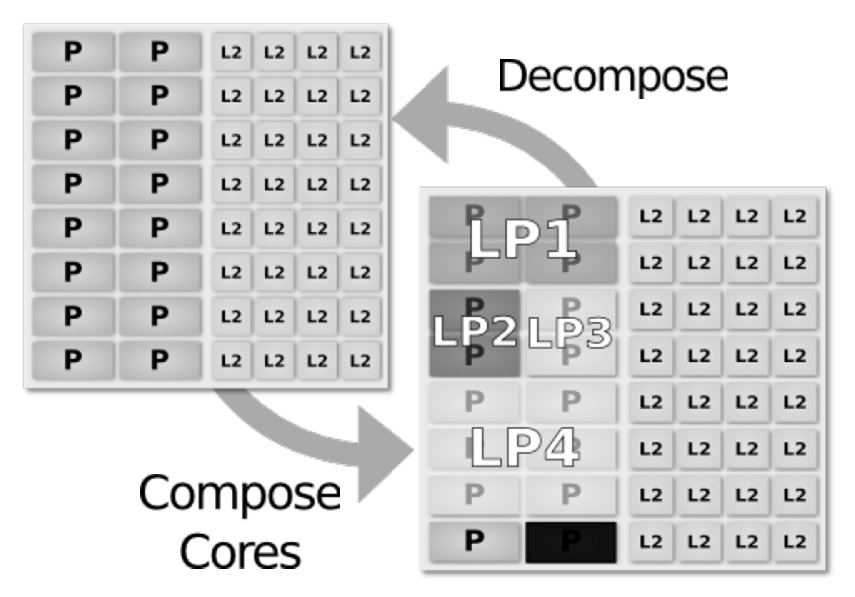
\includegraphics[width=0.3\textwidth]{graphics/dmcgraph.pdf}
    \caption{High-level view of a dynamic multicore processor considered in this paper.}
    \label{fig:dynmulticore}
\end{figure}

%Explain the figure
In this paper we consider a dynamic multicore processor which allows cores to compose their execution resources, register files and private L1 caches to create logical processors to accelerate a single thread.
Figure~\ref{fig:dynmulticore} shows a high-level view of the architecture and the two possible states: composed and decomposed.
The composed state represents a set of physical cores fused to create a larger logical core.
Multiple sets of cores can be fused to create logical cores of different sizes.
In Figure~\ref{fig:dynmulticore} for example, LP1 is composed of four physical cores whereas LP2 is composed of two.
At runtime, physical cores may be decomposed from a logical processor to remove them from the core composition.

\vspace{10mm}
\subsection{Streaming Programming Languages}

% % This section should explain what steaming programming is (remove all the details about each language)
% General purpose programming languages often propose very little support for programs that handle with a continuous flow of data.
% This results in having to design a set of complicated for loops to manage the streams of data.
% Having to deal with different rates of incoming and outcoming data also increases the complexity of writing these applications using a standard language.

Streaming programming languages are a branch of dataflow programming that focus on applications that deal with a constant stream of data.
These applications, such as audio or video decoding can be commonly found in mobile devices.
Unlike conventional programming languages such as C++, these languages abstract the concept of incoming and outgoing data to permit the programmer to focus on how the data should be treated.
Programs are described as directed graphs where nodes are functions and their edges represent their input and output streams. 
These languages offer primitives to describe such a graph~\cite{theis2002streamit} which expose parallelizable and serial sections of the application directly to the compiler. 
Rates of incoming and outcoming data can also be defined to facilitate load balancing optimizations~\cite{chen2005rawstream}.

Features of streaming programming languages make them an ideal language for targeting multicore processors.
The explicit data communication between the different tasks in the program, the ability to estimate the amount of work performed in each task and information about data rates between tasks allows the compiler to easily generate a multi-threaded application that can run on a dynamic multicore processor.
However, the main challenge consists of deciding how to map the different tasks onto threads and how to allocate the right amount of resources to maximize performance.



\section{Motivation}
\label{sec:motiviation}
\begin{figure}[t]
    \centering
    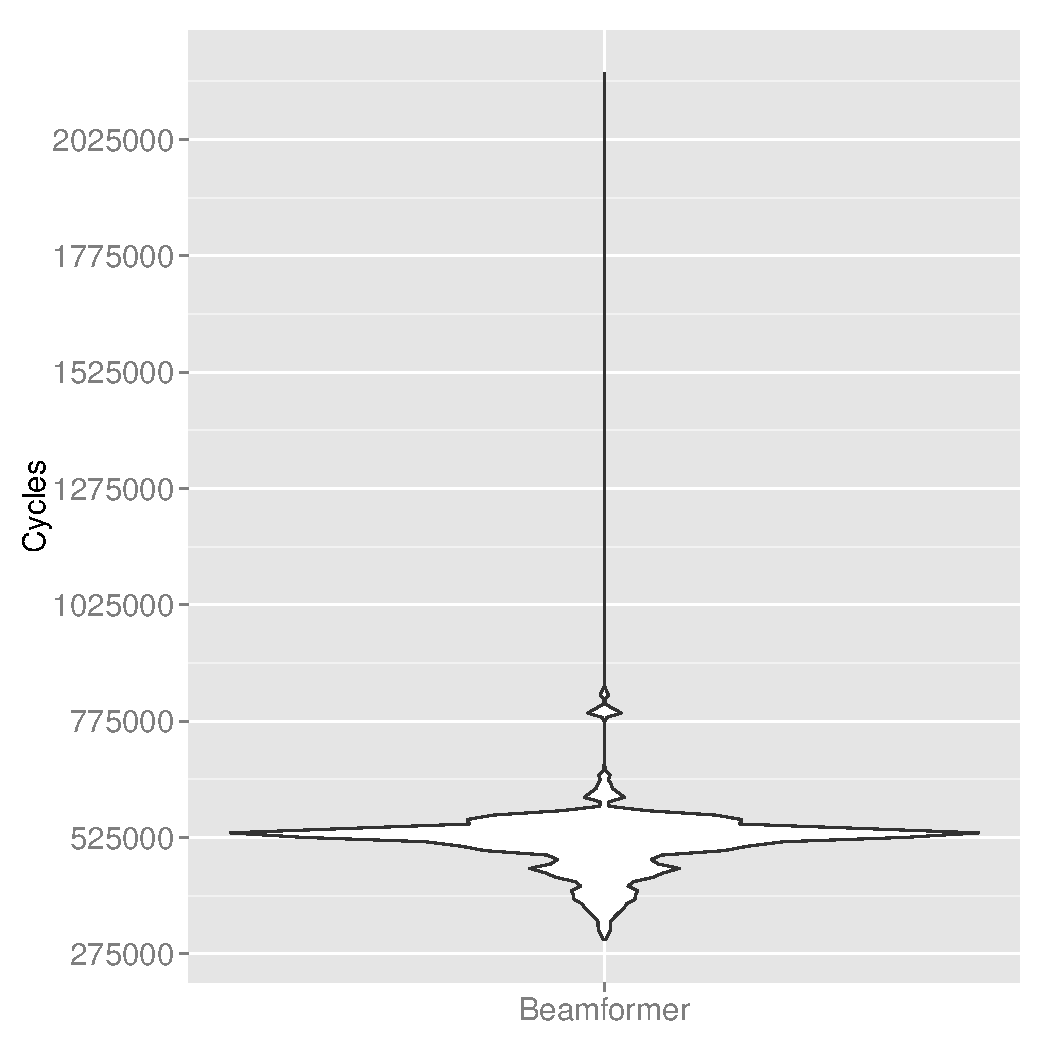
\includegraphics[width=1\textwidth]{streamit-paper/graphics/beamformer_motivation.pdf}
    \caption{Distribution of the runtime for Beamformer resulting from an exhaustively exploration of the hardware/software co-design space.
     The application has been partitioned into different number of threads and core compositions.}
     \label{fig:beamformermotiv}
\end{figure}

This section illustrates the difficulty of finding a good partition and resource allocation.
A simple experiment is conducted where one StreamIt benchmark is taken, \bench{Beamformer}, and partition its tasks into threads and allocate various number of cores to each thread.
A co-design of more than 32,000 combinations (exhaustive space) of thread mappings and core compositions is generated.
Each design point is executed on a dynamic multicore simulator (exact details about the experimental setup are presented later in section~\ref{sec:setup}).

Figure~\ref{fig:beamformermotiv} presents the distribution of the execution times from the co-design space as a violin plot.
For the unfamiliar reader, an intuitive way to think about this violin plot is to consider it as a smoothed histogram rotated by 90 degrees and mirrored.
The majority of the sampled points have a cycle count around 525,000 with the worst points taking more than 2 millions cycles.
The best performance is around 275,000 cycles which is about 2x faster than the majority of the data points.
This shows that finding the right combination of thread mapping and core composition is critical since a wrong choice often leads to suboptimal performance.

This example illustrates the necessity for designing the technique to predict both the optimal number of threads and core composition to use.
The next section will present a more in-depth analysis of the design space before presenting our machine-learning predictive model.



\section{Methodology}
\label{sec:setup}
This section describes the setup used throughout this chapter to conduct the design space exploration.
It starts by presenting the overall workflow and then explores briefly some of the features of the benchmarks.
Finally the section explains how the number of design points used throughout the exploration were determined.

\begin{figure}[t]
    \centering
    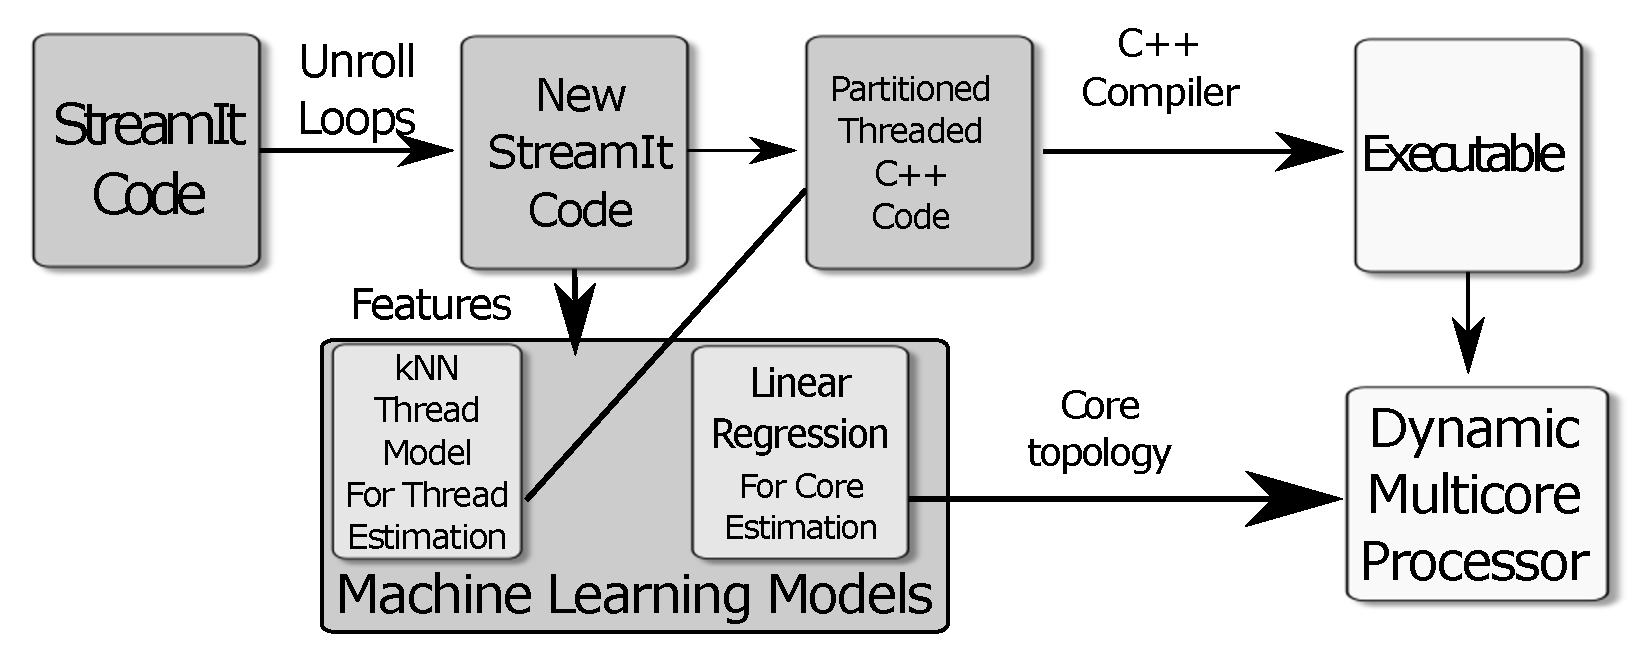
\includegraphics[width=1\textwidth]{streamit-paper/graphics/explanation3.pdf}
    \caption{Description of the workflow.
    Two distinct machine-learning models are used to predict the optimal thread partitioning and core composition based on static code features.}
    \label{fig:overview}
\end{figure}

\subsection{Overview}

\begin{figure}[t]
    \centering
    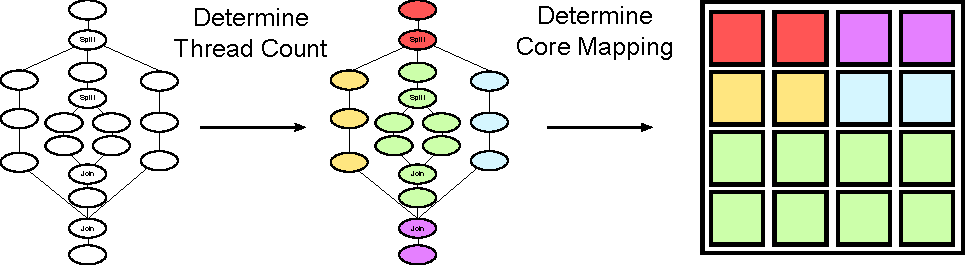
\includegraphics[width=1\textwidth]{streamit-paper/graphics/examplestrem.pdf}
    \caption{Example of a StreamIt program being partitioned into threads (represented by the different colours) followed by assigning cores to each thread.}
    \label{fig:examplestream}
\end{figure}

Figure~\ref{fig:overview} presents the workflow of the system used in this chapter and Figure~\ref{fig:examplestream} illustrates the workflow on a synthetic StreamIt graph.
First, the source-to-source StreamIt compiler is used to unroll loops as this is often beneficial when cores are composed as will be seen later in Section~\ref{sec:streamit:dse}.
Then, static code features such as the program's graph structure are extracted from the StreamIt code through the StreamIt source-to-source compiler.
These features are used as an input to the first machine-learning model that determines how many threads will be required based on an estimate of Thread Level Parallelism (TLP) found in the program.
This information is used to partition the program into threads which is done by the StreamIt compiler which produces a C++ program using pthreads.
This is exemplified in Figure~\ref{fig:examplestream}, the colours filling in the nodes represent the threads each node has been assign to.
This C++ program is then compiled using the compiler for EDGE described in Chapter~\ref{chp:setup} Section~\ref{chp:setup:comp}.

Then, a second machine-learning model is deployed which also analyses static code features extracted from the SteamIt code, once again provided by the source-to-source compiler.
This model decides on the number of cores each thread will have.
This is achieved by estimating the amount of Instruction Level Parallelism (ILP) that can be possibly extracted in each thread and by determining how many physical cores should be fused for that thread.
Finally, the processor is reconfigured to compose the requested resources ahead of time and execute the partitioned program.
For example in Figure~\ref{fig:examplestream}, once the graph is coloured, the machine learning model estimates the potential ILP in each group and assigns a number of cores each thread will execute on.

\subsection{Design Space}

The benchmarks used throughout this chapter are shown in Chapter~\ref{chp:setup} Section~\ref{chp:setup:streamit}.
These applications represent a variety of embedded applications and kernels, from digital signal processing to a matrix-multiplication kernel or band pass filters.
Table~\ref{tab:instancefilt} shows the number of filter instances and SplitJoins for each of the benchmarks.
As a refresher from Chapter~\ref{chp:Background} Section~\ref{chp:bckg:streamit}, SplitJoin filters are functions which distribute and collect data from parallel filters.
The applications feature a different number of SplitJoins which determine the task-level parallelism.
This is to include a variety of situations to test the flexibility of the dynamic multicore processor.
Whilst SplitJoins often facilitate the decision of how to partition the programs into threads, they are not the only way to exploit thread level parallelism.
The applications which do not feature SplitJoins can still be split into threads and will operate in a pipelined fashion~\cite{theis2002streamit}.
For each benchmark the default inputs provided in the repository~\cite{streamitrepo} are used and the default iteration count is set to 10. 

\begin{table}[t]
% The FFT need are variable
  \small
 \begin{tabular} { | l | l | l | l | l | l | }
 \hline
 \cellcolor[gray]{0.7}Type  & \cellcolor[gray]{0.7}Audiobeam&  \cellcolor[gray]{0.7} Beamformer& \cellcolor[gray]{0.7}Bitonic-Sort  &  \cellcolor[gray]{0.7} BubbleSort &  \cellcolor[gray]{0.7}  CFAR\\ \hline
  Filter Instances & 18 & 56 & 82 & 18 & 3 \\ \hline
	\# of SplitJoins &	1 & 2 & 44 & 0 & 0 \\ \hline

 \cellcolor[gray]{0.7}Type  & \cellcolor[gray]{0.7}ChannelVocoder &  \cellcolor[gray]{0.7} FFT&  \cellcolor[gray]{0.7}FFT3 &  \cellcolor[gray]{0.7} FFT6&  \cellcolor[gray]{0.7}FilterBank \\ \hline
  Filter Instances & 53 & 20 & 185 & 99 & 67 \\ \hline 
   \# of SplitJoins &	 1 & 12 & 44 & 96 & 9 \\ \hline 

   \cellcolor[gray]{0.7}Type& \cellcolor[gray]{0.7}FIR &  \cellcolor[gray]{0.7} FMRadio &  \cellcolor[gray]{0.7} InsertionSort &  \cellcolor[gray]{0.7} Matmul-Block &  \cellcolor[gray]{0.7} RadixSort\\ \hline
  Filter Instances& 131 & 29 & 6 & 4 & 13 \\ \hline
  \# of SplitJoins&    0 & 7 & 0 & 7 & 0 \\ \hline

 \end{tabular}
  \caption{Number of filter instances and SplitJoin filters present in each benchmark.}\label{tab:instancefilt}
\end{table}

%\begin{table}[t]
% The FFT need are variable
 % \small
 %\begin{tabular} { | l | l | l | l | l | }
 %\hline
 %  \cellcolor[gray]{0.7}Audiobeam&  \cellcolor[gray]{0.7} Beamformer& \cellcolor[gray]{0.7}Bitonic-Sort  &  \cellcolor[gray]{0.7} BubbleSort &  \cellcolor[gray]{0.7}  CFAR\\ \hline
 % 1 & 2 & 44 & 0 & 0 \\ \hline
 %  \cellcolor[gray]{0.7}ChannelVocoder &  \cellcolor[gray]{0.7} FFT&  \cellcolor[gray]{0.7}FFT3 &  \cellcolor[gray]{0.7} FFT6&  \cellcolor[gray]{0.7}FilterBank \\ \hline
 % 1 & 12 & 44 & 96 & 9 \\ \hline 
 %  \cellcolor[gray]{0.7}FIR &  \cellcolor[gray]{0.7} FMRadio &  \cellcolor[gray]{0.7} InsertionSort &  \cellcolor[gray]{0.7} Matmul-Block &  \cellcolor[gray]{0.7} RadixSort\\ \hline
 % 0 & 7 & 0 & 7 & 0 \\ \hline
% \end{tabular}
%  \caption{Number of split joins present in each benchmark.}\label{tab:splitjoin}
%\end{table}

\begin{table}[t]
\centering
\begin{tabular} { p{5.2cm}  p{1.8cm} }
      \toprule
      \textbf{Parameter} & \textbf{Values} \\ \midrule
      \# of cores in the processor & 16 \\
      \# threads per application & 1 -- 15 \\
      \# cores per thread & 1 -- 15 \\ \midrule
      \# sampled core compositions & 100 \\ 
      \# our sampled space & 1316 \\
      \# total sample space & 32767 \\ \bottomrule
    \end{tabular}
  \caption{Design space considered per application.}
  \label{tab:space}
\end{table}

The parameters and size of the space are given in Table~\ref{tab:space}.
In this study the 16 core DMP defined in Chapter~\ref{chp:setup} Section~\ref{chp:setup:conf} is used.
Having 16 cores allows for a larger variety of configurations, this also represents a processor similar to a tiled embedded system such as Tilera or Raw.
All cores in the DMP are utilised; Core 0 is assigned to the main thread and for runtime management.
This leaves 15 cores available for each application.
Each core is restricted to running only a single thread, as no context switching is supported, which leads to a possible number of threads between 1 and 15.
The core-composition is not used on the master core, leaving 15 physical cores to be distributed to each of the worker threads.
Cores can be composed together to form a composition with up to 15 physical cores, making the total number of cores assigned to a thread between 1 and 15.
Of course, not all cores have to be assigned to a thread, in this case all remaining cores that aren't in a composition or a thread are turned off.
Overall, this leads to a total space size of 32,767 unique combination per benchmark as previously described in Section~\ref{sec:motivation}.

\subsection{Sample Space}

Given a partition, any benchmark that can be split into 15 threads requires 32,767 executions to cover the entire space.
Running the exhaustive exploration of the space for a benchmark requires approximately a week of simulation on a 572+ node supercomputer.
For this reason, a sample of 1,316 random points from the entire space is utilised.
This roughly corresponds to 100 core compositions for each number of threads; the actual number, 1,316 is smaller than 1,500 since for low and high thread counts there are less than 100 possible different core composition.
For example, a single thread can have only up to 15 different core-compositions (1 through 15) whilst 15 threads can only have a single core given to each thread.
\bench{InsertionSort} is the only exception since it can at most only be split into 5 threads leading to 415 sample points.
Overall, the space exploration required one week of simulation on the supercomputer~\cite{ecdf}.

\begin{figure}[t]
  \centering
    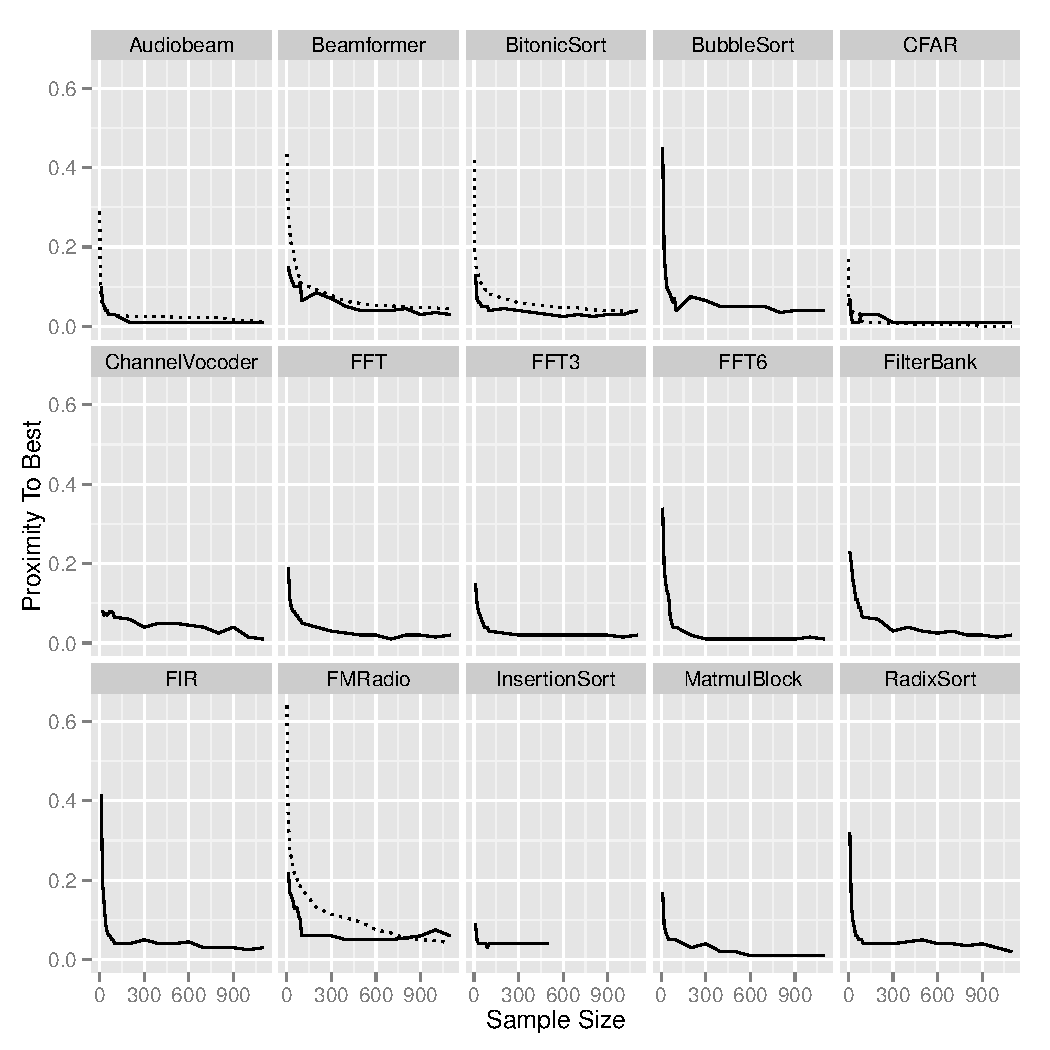
\includegraphics[width=1\textwidth]{streamit-paper/graphics/ESCProx.pdf}
    \caption{Statistical (plain line) and actual proximity (dotted line, this is only done for 5 benchmarks) to best performance using a subset of the sample space.}\label{fig:prox}
\end{figure}

%Define stopping criterion?
To gain confidence that the best configuration from the sample space is indeed close to the real best in the entire space, a statistical model based on the Early Stopping Criterion defined in~\cite{vuduc2003AutomaticPerf} is deployed.
This statistical model estimates, given a sample of the total space, if the best observed performance of that sample space is within a percentage of the statistical best performance, a more detailed explanation can be found in Chapter~\ref{chp:Background} Section~\ref{sec:esc}.
The results demonstrate that the sample space selected is representative of the whole space.

Figure~\ref{fig:prox} shows, for each of the benchmarks, the proximity to the statistical best when increasing the sub-sample space given a maximal uncertainty of 5\%  (\ie minimum 95\% confidence).
As can be seen by the plain line, the model shows that the best sample point is actually within 5\% (0.05 proximity) of the best for all the benchmark.
The proximity is measured by taking the best currently observed point and comparing it to the latest discovered point.
To further prove that the statistical model based on the Stopping Criterion is indeed accurate, an exhaustive exploration of five benchmarks is conducted.
The dotted line in figure~\ref{fig:prox} shows the actual proximity to the best for \bench{Audiobeam}, \bench{Beamformer}, \bench{BitonicSort}, \bench{CFAR} and \bench{FMRadio}.
As can be seen after 1316 samples, the achieved performance is actually very similar to the one predicted by the statistical model, hence confirming prior work~\cite{vuduc2003AutomaticPerf}.
To summarise, it can be concluded that the best point found in the sample space of 1,316 points is at least within 5\% of the real best in the exhaustive space with 95\% confidence.

\subsection{Synthetic Benchmarks}

\begin{table}[t]
% The FFT need are variable
  \small
 \begin{tabular} { | l | l | l | }
 \hline
 & Av. Number of SplitJoins & Average Number of Filter Instances \\ \hline
 Selected Benchmarks & 14 & 52 \\ \hline 
 Synthetic & 22 & 64 \\ \hline
 \end{tabular}
 \caption{Data on the synthetic benchmarks compared to the selected benchmarks}~\label{tab:synthvsreal}
 \end{table}

One of the difficulties of building a machine learning based model for StreamIt is the lack of a large amount benchmarks available~\cite{wang2013partitionstreamit}.
To overcome this problem generating synthetic benchmarks can be a solution~\cite{cumminsopencl2017}.
Thus synthetic StreamIt benchmarks are generated and statistics are gathered from them in a similar style as in~\cite{wang2013partitionstreamit}.
In this chapter, the synthetic benchmarks are used to build a model for predicting the number of threads, which will be described later in section~\ref{sec:ml}

%Cite repository
To ensure that the synthetic benchmarks are representative of realistic benchmarks they are created using filters from a set of example StreamIt programs found in the example directory in the repository.
30 different possible filters with different incoming and outgoing rates and different inputs and outputs types are used to increase the variety of the dataset.
To ensure that the synthetic benchmarks are similar to real benchmarks, the total number of filters and split joins are within the average of the realistic benchmarks.
Table~\ref{tab:synthvsreal} gives the average number of SplitJoins and filter instances for the synthetic benchmarks vs the real benchmarks used in this chapter.
As can be seen, the synthetic benchmarks, on average, have more SplitJoins than the real benchmarks; this is due to the fact that a few of the benchmarks presented in the chapter don't have SplitJoins at all which can quickly reduce the average.
%Maybe say a bit more here.
Since these benchmarks are built to be used for predicting the number of threads an application should use, and SplitJoins are explicit declarations of task-level parallelism, having a higher average number of SplitJoins is not detrimental to building the model.


\section{Design Space Exploration}
\label{sec:streamit:dse}
This section describes the exploration of the software/hardware co-design space.
The software side includes partitioning the program, determining the number of threads and the specific source-level optimisations.
The hardware side is about finding out the best core composition that maximizes performance for a given partitioning.

\subsection{Thread Partitioning}

This section first starts with analyzing the impact of thread partitioning on performance.
In this section, the term optimal number of threads defines the number of threads which results in the best performance for any given benchmark.
Thread partitioning is about deciding how many threads to create and how to partition StreamIt filters into these threads.

To simplify this study, the default streaming partitioner is used to decide on how to allocate filters to threads which is based on simulated annealing~\cite{simulatedAnnealing1983}.
On the hardware side, two scenarios are considered: the ``without composition scenario'' where there is exactly one core per thread and the ``with composition scenario'' where each thread receives between 1 and 15 cores.
Figure~\ref{fig:threadtrend} shows how performance varies under both scenarios as a function of the number of threads.
In this figure, the ``with composition scenario`` uses points from the sample space that result in the fastest execution time for a given number of threads.
Regardless of how cores are composed it can be observed that curves for a benchmark follow the same trend.
As can be seen in Figure~\ref{fig:threadtrend}, the optimal number of threads using core composition is very similar to the scenario without composition as both curves follow the same performance trends.
This is due to the fact that StreamIt is oriented towards task-level parallelism and thus, multithreading will be a natural fit for performance improvements whilst core-composition may have less of an effect overall.
As Figure~\ref{fig:threadtrend} shows that the performance trends for both with and without composition are similar when it comes to thread counts, this  means that the optimal number of threads for a benchmark can be estimated independently from the hardware composition.
The system can therefore proceed in two stages: first determine the optimal number of threads and then decide on a core composition.

Figure~\ref{fig:threadtrend} also shows that the performance of most benchmarks starts to deteriorate passed a certain number of threads making it critical to not over-allocate threads.
This number of threads varies between benchmarks, thus it motivates the use of machine learning to decide the optimal number of threads to use.
Finally it is important to observe that executions without compositions always perform worse.
This demonstrates that composing cores is essential to obtain the best performance from a workload.


\subsection{Core Composition}

\begin{figure}[t]
  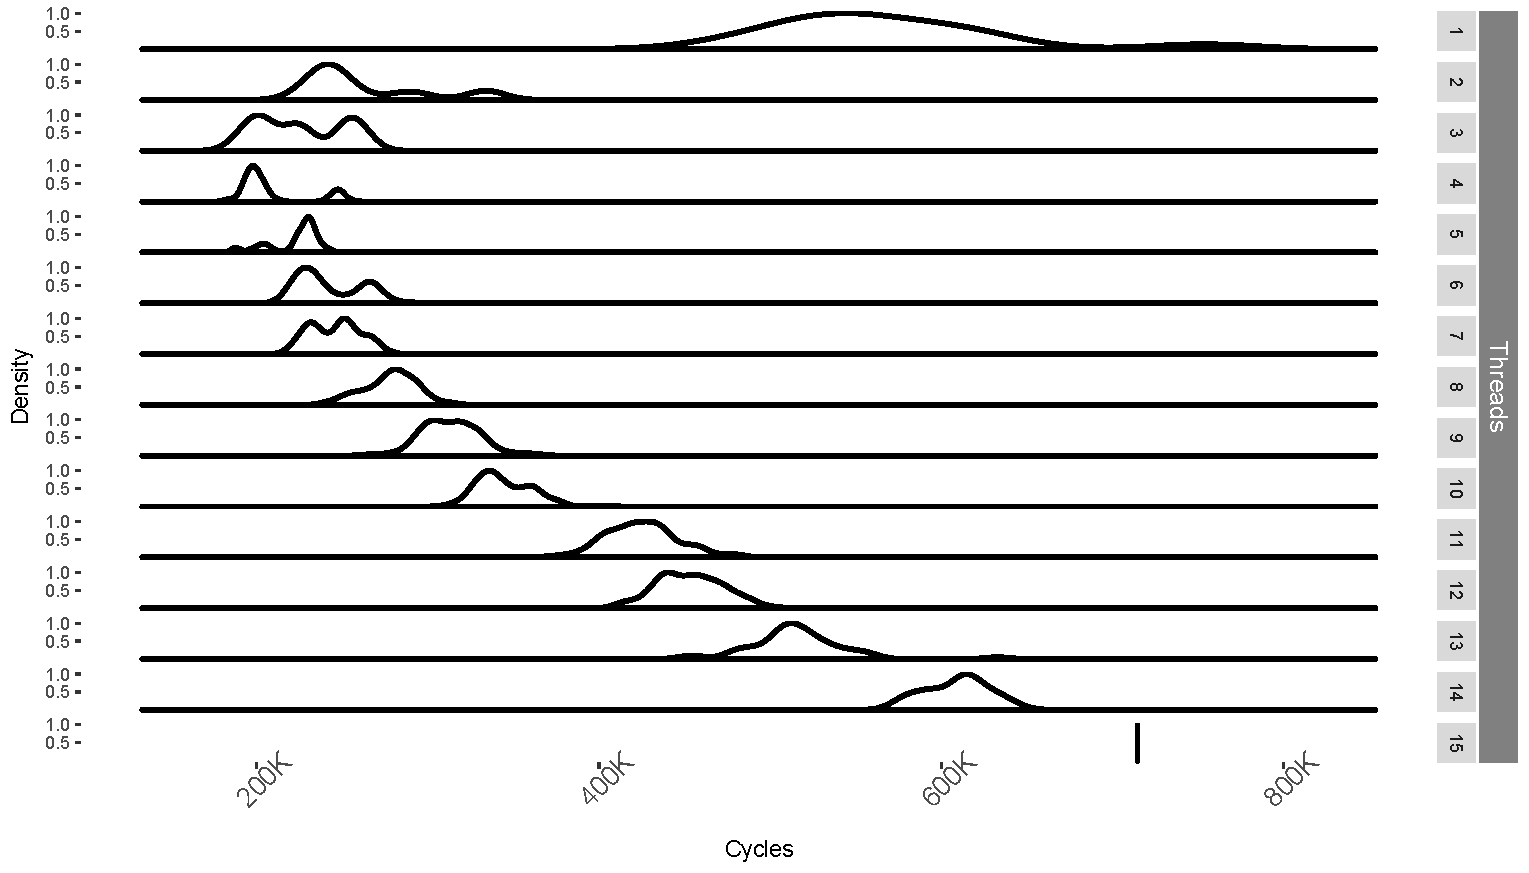
\includegraphics[width=1\textwidth]{streamit-paper/graphics/filterbank_tot.pdf}
  \caption{Distribution of FilterBank performance when modifying the amount of threads and compositions.}\label{fig:fbtotal}
\end{figure}

Using core composition, the processor fuses a number of cores and associates them to a thread to increase the thread's performance.
Whilst this flexibility is advantageous, choosing the right amount of cores for a given thread is difficult due to the large number of possible configurations~\cite{gulati2008multitaskingdmc}.

Figure~\ref{fig:fbtotal} shows how threading and core-compositions affect performance for the \bench{FilterBank} benchmark.
The curves represent the density distribution for different core compositions as a function of the number of threads.
The right hand side Y-axis represents the number of threads present in the current version of the benchmark whilst the left Y-Axis represents the density normalized by the total number of points in the design space.
For each of the threaded versions the benchmark runs using 100 different core-compositions.
The density curve for thread 15 is a single point as there exists only a single composition, so a line is drawn to represent where that point lies.

The width of each of the curves represents the influence of composition on the \bench{FilterBank}'s performance for a given number of threads.
For this benchmark, the impact of having core-composition enabled often leads to a 1.5x speedup compared to running only in multi-threaded mode; this can be seen for 1 to 4 threads.
Interestingly, as more threads are used, performance worsens, echoing the results shown in the previous section.
This is due to the fact that when the number of threads is increased, synchonization between threads will increase whilst the potential number of corse which can be fused decreases.
In the case where the application does not feature highly parallel tasks, de-prioritising core compositions can negatively impact performance.
This signifies that for the benchmark \bench{FilterBank}, it is more important to fuse cores with a small amount of threads rather than add more and more threads to the application.


\begin{figure}[t]
  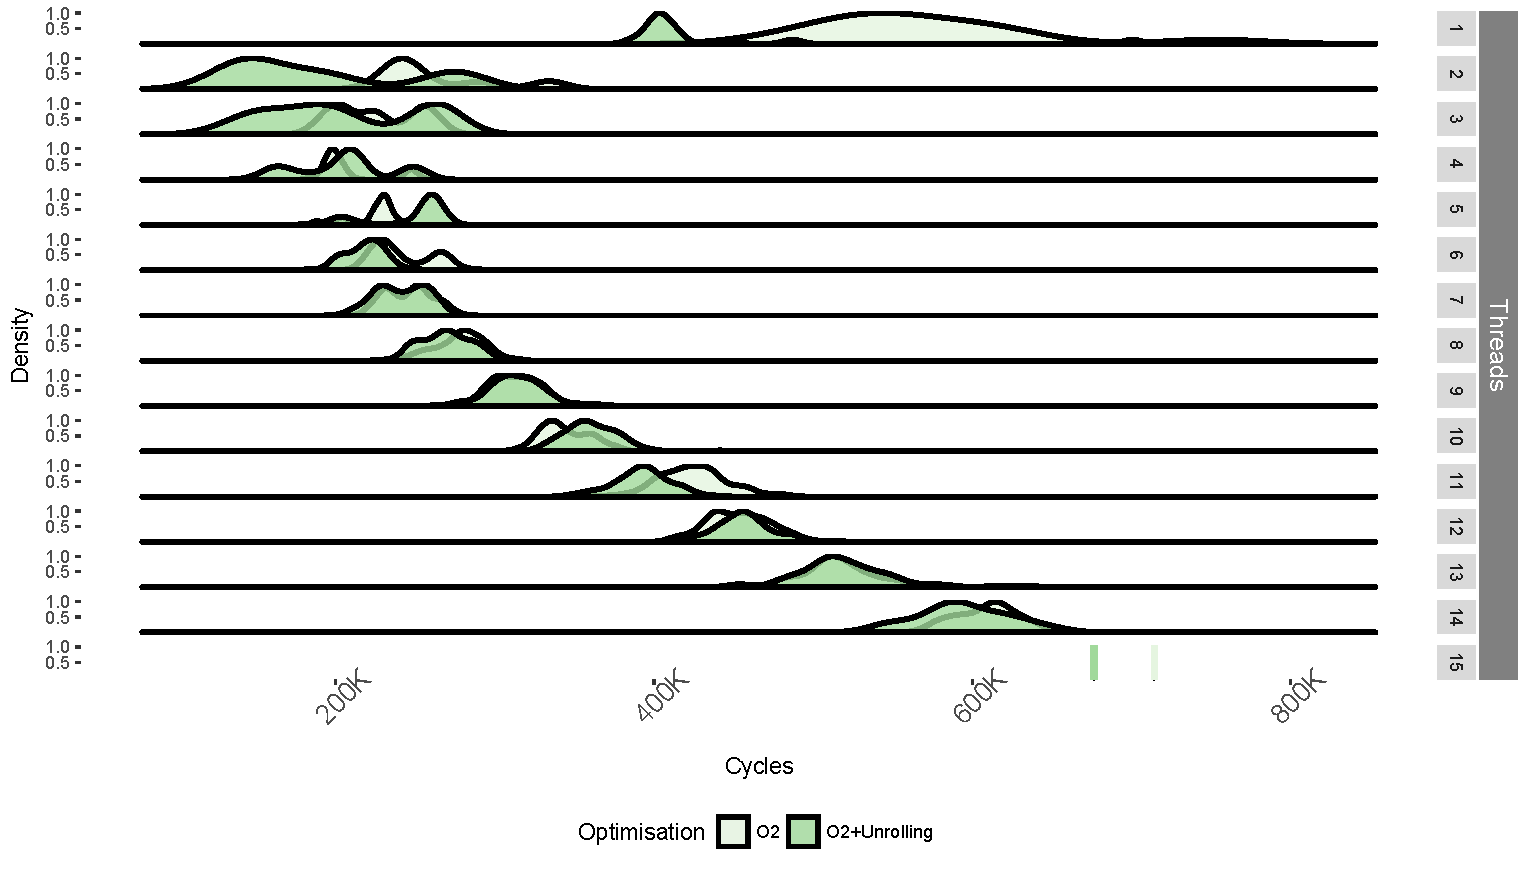
\includegraphics[width=1\textwidth]{streamit-paper/graphics/filterbank_unroll.pdf}
  \caption{Distribution of FilterBank performance when modifying the amount of threads, composition and unrolling factor.}\label{fig:fbunroll}
\end{figure}


\subsection{Impact of Loop Transformation}
As seen in Chapter~\ref{chp:Background}, composing cores exploits block-level parallelism by running multiple EDGE blocks on a logical core.
As physical cores in a logical core must communicate to submit block address predictions, and commit information to each other, having a small number of blocks will reduce the communication overhead.
In a core-composition, commit information can be a core informing another core that it has become the non-speculative core, or that registers can be read or written to.
Since physical cores can fetch more than a single block when the blocks are made of a small number of instructions, if the program being executed is comprised of small blocks this will cause a composition to fetch a high amount of blocks.
Thus finding methods to increase the average size of the blocks can lead to reduced overhead.
One method of increasing the size of the blocks is through loop unrolling.
This section therefore analyses the impact of loop unrolling on the StreamIt benchmarks.

In this Chapter, unrolling is done at the source level via a flag passed to the StreamIt source-to-source compiler.
Given a number of times the loops must be unrolled, the StreamIt source-to-source compiler will generate the multi-threaded C++ code with the loops unrolled.
Figure~\ref{fig:fbunroll} presents an example of how loop unrolling affects performance on the \bench{FilterBank} benchmark.
The graph presents the same information as Figure~\ref{fig:fbtotal} but comparing .
Figure~\ref{fig:fbunroll} shows that unrolling loops for \bench{FilterBank} can improve performance by up to 1.42x compared to the fastest non-unrolled version.
Another observation is that the best execution times for each of the threaded versions when unrolling does not follow the same trend seen in Figure~\ref{fig:threadtrend}.
The leftmost curve performance peaks at two threads whereas the rightmost peaks at 3 compared to 4 in the non-unrolled version.

\begin{figure}[t]
  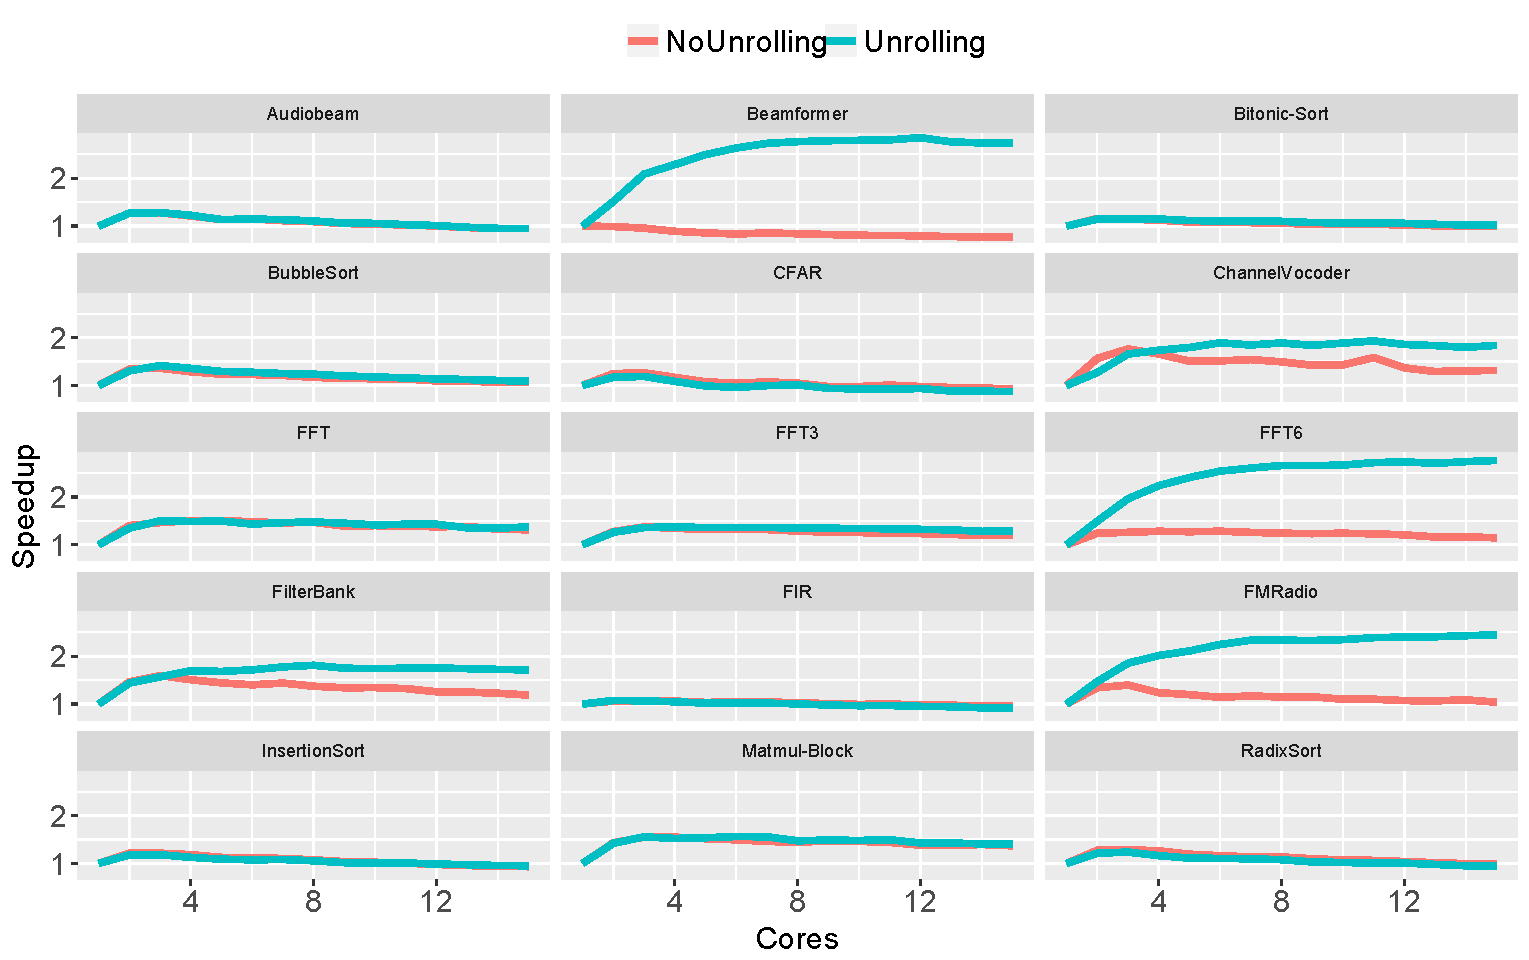
\includegraphics[width=1\textwidth]{streamit-paper/graphics/unrolling_vs_no_single_core.pdf}
  \caption{How unrolling affects how much performance can be obtained via core-composition on the single-threaded versions of each benchmarks.}\label{fig:unroll_summary}
\end{figure}

Figure~\ref{fig:unroll_summary} goes into more details on how unrolling affects the amount of speedup obtained by running each of the StreamIt benchmarks on a single thread using different number of cores in the composition.
In this figure, the X axis represents the number of cores in the composition, ranging from single core to 15.
The Y axis compares the execution time in number of cycles for the benchmark using a single core vs a given core-composition.
The colours of the lines represent with and without unrolling.
As can be seen, for the set of benchmarks used throughout this chapter, five benchmarks benefit from unrolling.
These benchmarks are \bench{Beamformer}, \bench{ChannelVocoder}, \bench{FFT6}, \bench{FilterBank} and \bench{FMRadio}. 

\begin{figure}[t]
  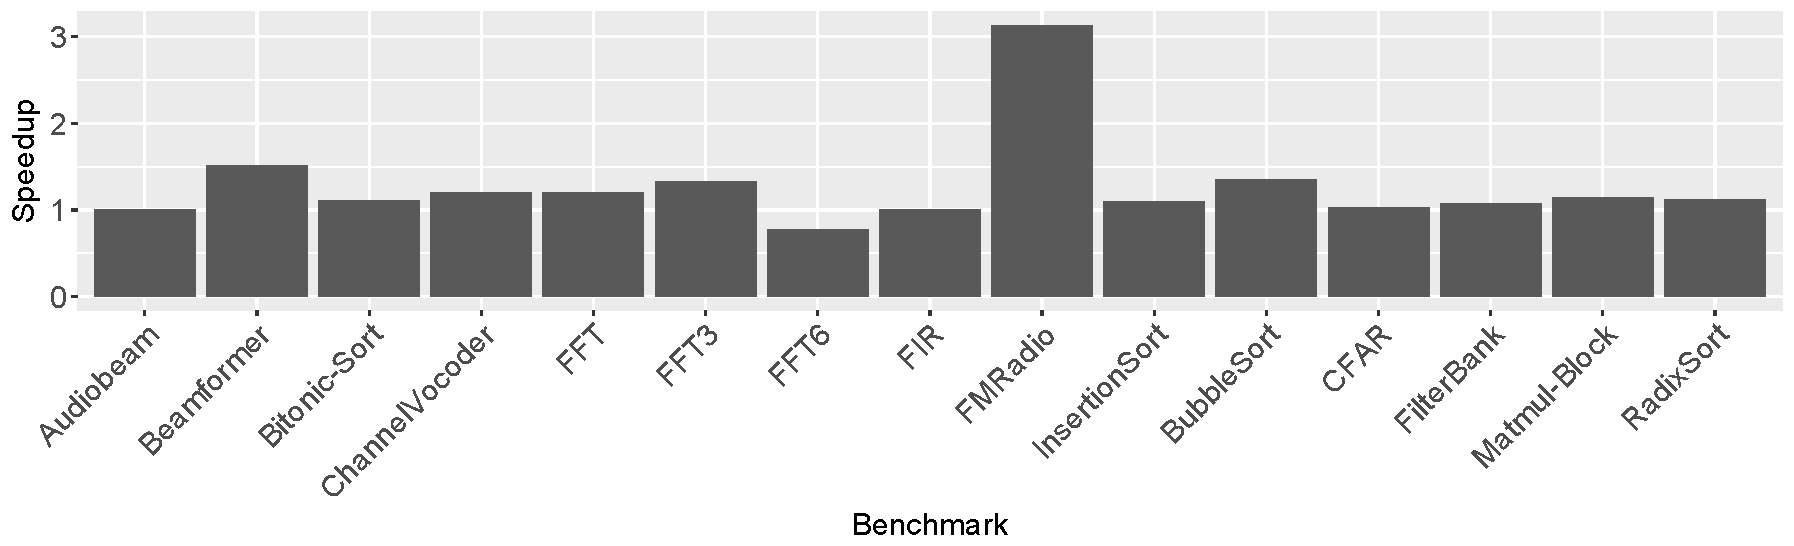
\includegraphics[width=1\textwidth]{streamit-paper/graphics/unroll_speed_bars.pdf}
  \caption{Speedup obtained .}\label{fig:unroll_bars}
\end{figure}
Figure~\ref{fig:unroll_bars} complements Figure~\ref{fig:unroll_summary} by showing the speedup obtained by unrolling loops when executing the benchmark on a single core.
On average, the information shown in Figure~\ref{fig:unroll_bars} coincides with the data shown in Figure~\ref{fig:unroll_summary}: benchmarks that don't scale also see no difference in performance when loop unrolling is called.
For the benchmarks that do not scale with unrolling; this is most certainly due to the for loops containing conditional statements which may keep the blocks size small.
When a loop that holds multiple conditional statements is unrolled, conditional statements may not be fused into a single block; thus the block size does not change.
Benchmark \bench{FMRadio} sees a 3x improvement compared to the non-unrolled version, this is due to the fact that all the loops are fully unrolled, reducing the total number of instructions required to execute the task.
For the \bench{FFT6} benchmark, unrolling loops will actually cause the single-core version to be slower than its not unrolled version.
%I think this is due to a refreshing performance thing
This is due to the fact that for \bench{FFT6}, the source to source unrolling adds intermediate variables in the loop which increase the number of loads and stores.
Whilst it may be slower on a single core, as seen in Figure~\ref{fig:unroll_bars}, having a core-composition running the thread will still result in faster execution that without loop-unrolling.

Figure~\ref{fig:unroll_size} shows the influence of loop unrolling on the average size of an EDGE block for each of the benchmarks.
The size represents the number of instructions exected in each of the EDGE blocks.
As can be seen, the data for \bench{Beamformer} and \bench{FFT6} in Figure~\ref{fig:unroll_size} corroborate with the idea that larger block sizes will result in better performance when fusing cores.
However whilst benchmarks \bench{ChannelVocoder}, \bench{FilterBank} and \bench{FMRadio} also see an increase in blocksize, it is not as important and averages out at a 1.22x increase.
%Be clearer here.
That said, even a small amount of increase can help improve the scalability of core-composition.

\begin{figure}[t]
  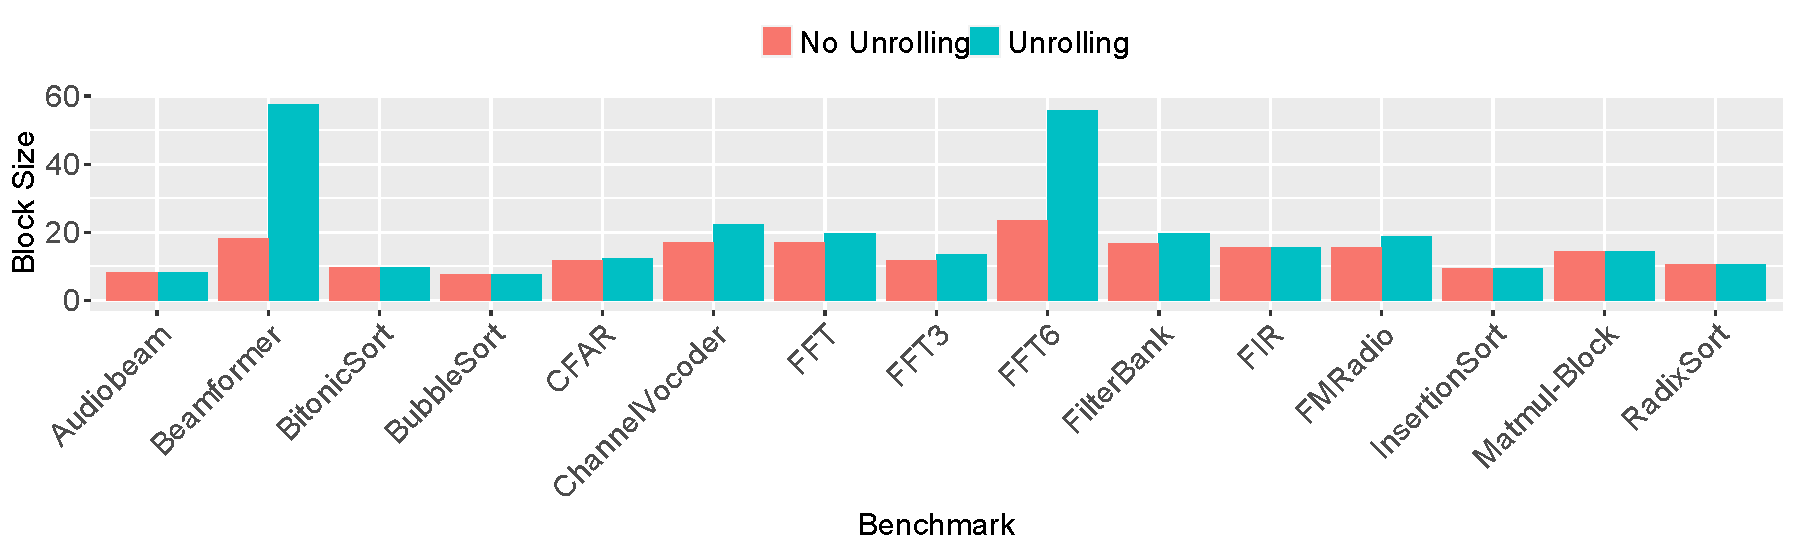
\includegraphics[width=1\textwidth]{streamit-paper/graphics/unrolling_size.pdf}
  \caption{Average size (in instructions) of blocks executed with and without unrolling for each benchmark .}\label{fig:unroll_size}
\end{figure}

Overall, this section has shown that loop unrolling can improve performance by increasing the size of blocks for the benchmarks which helps improve the efficiency of core-compositions.

\subsection{Co-Design Space Best Results}


This section  presents the results of the entire co-design space exploration.
Figure~\ref{fig:overviewhist} characterizes how much of a performance increase, over a baseline of a single-core single-thread with O2 optimisations, can be obtained with and without unrolling.
For each benchmark, the \textit{THREAD} bar represents the maximal speedup obtained by dividing the program into threads without fusing cores.
The \textit{CORE} bar represents the best speedup when the benchmark is executed in a single thread and fuse cores.
\textit{BOTH} represents the best speedup obtained for each benchmark using a combination of \textit{THREAD} and \textit{CORE}.
Finally, for each benchmark, the results are obtained for both an unrolled and not unrolled version to compare how the compiler optimisation affects performance.
Figure~\ref{fig:overviewhist} shows that when loops are not unrolled, composing cores will not greatly improve performance.
This is due to the fact that the amount of ILP found in filters without the unrolling is too little for there to be any benefit of composing cores.

In the scenario where there are no specific optimisations for composition, multithreading will be the main source of performance.
This can be seen when studying the geometric mean,without unrolling.
Finding the optimal number of threads gives a speedup of 1.92 compared to 1.33 when using only core composition, which is an improvement of 44\%.
This changes when taking unrolling into account as the core compositions can be used more efficiently.
In this case, the speedup obtained from only composing cores is only 13\% worse than using only threads.
For the \bench{FMRadio} benchmark, unrolling makes using only core-composition better than only using threads.
This information corroberates with the data seen in Figure~\ref{fig:unroll_summary}; it presents a unique case where the effect of core composition is important enough to change the dominant performance enhancer.
The performance increase obtained via the source-level loop unrolling via the compiler demonstrates that some modifications to the code must be done to ensure optimal use of the dynamic multicore processor.
%Thus loop unrolling demonstrates that the StreamIt programs must be modified to take advantage of the core composition.

Overall the results demonstrate that multi-threading is the prevalent leader of performance, even with unrolling turned on.
This is natural as StreamIt applications are naturally geared towards TLP as most programs have at least one SplitJoin as seen in the Table~\ref{tab:splitjoin} which gives the number of split-joins per benchmark.
Benchmarks with SplitJoins will naturally benefit from splitting the program into threads~\cite{thiesStreamit2010}.
%Make sure this is 100% true but as far as I remember this is the case
Those that do not feature SplitJoins can still be parallelised by splitting a Pipeline into multiple parts.
For example, benchmark \bench{FIR} features no SplitJoins, yet splitting the Pipeline in 2 will result in a 1.40x speedup.
However, it is important to note that whilst finding the optimal thread mapping may result in higher performance improvements than finding the optimal composition for a single thread, the best performance is always obtained through a combination of both optimizations.
For cases such as \bench{BeamFormer} the optimal pairing results in a 1.8x speedup compared to simply finding the best multit-threaded version.
On average, the optimal combination leads to a 1.5x performance increase compared to only multithreading.

\begin{landscape}
\begin{figure}\hspace{-1em}
    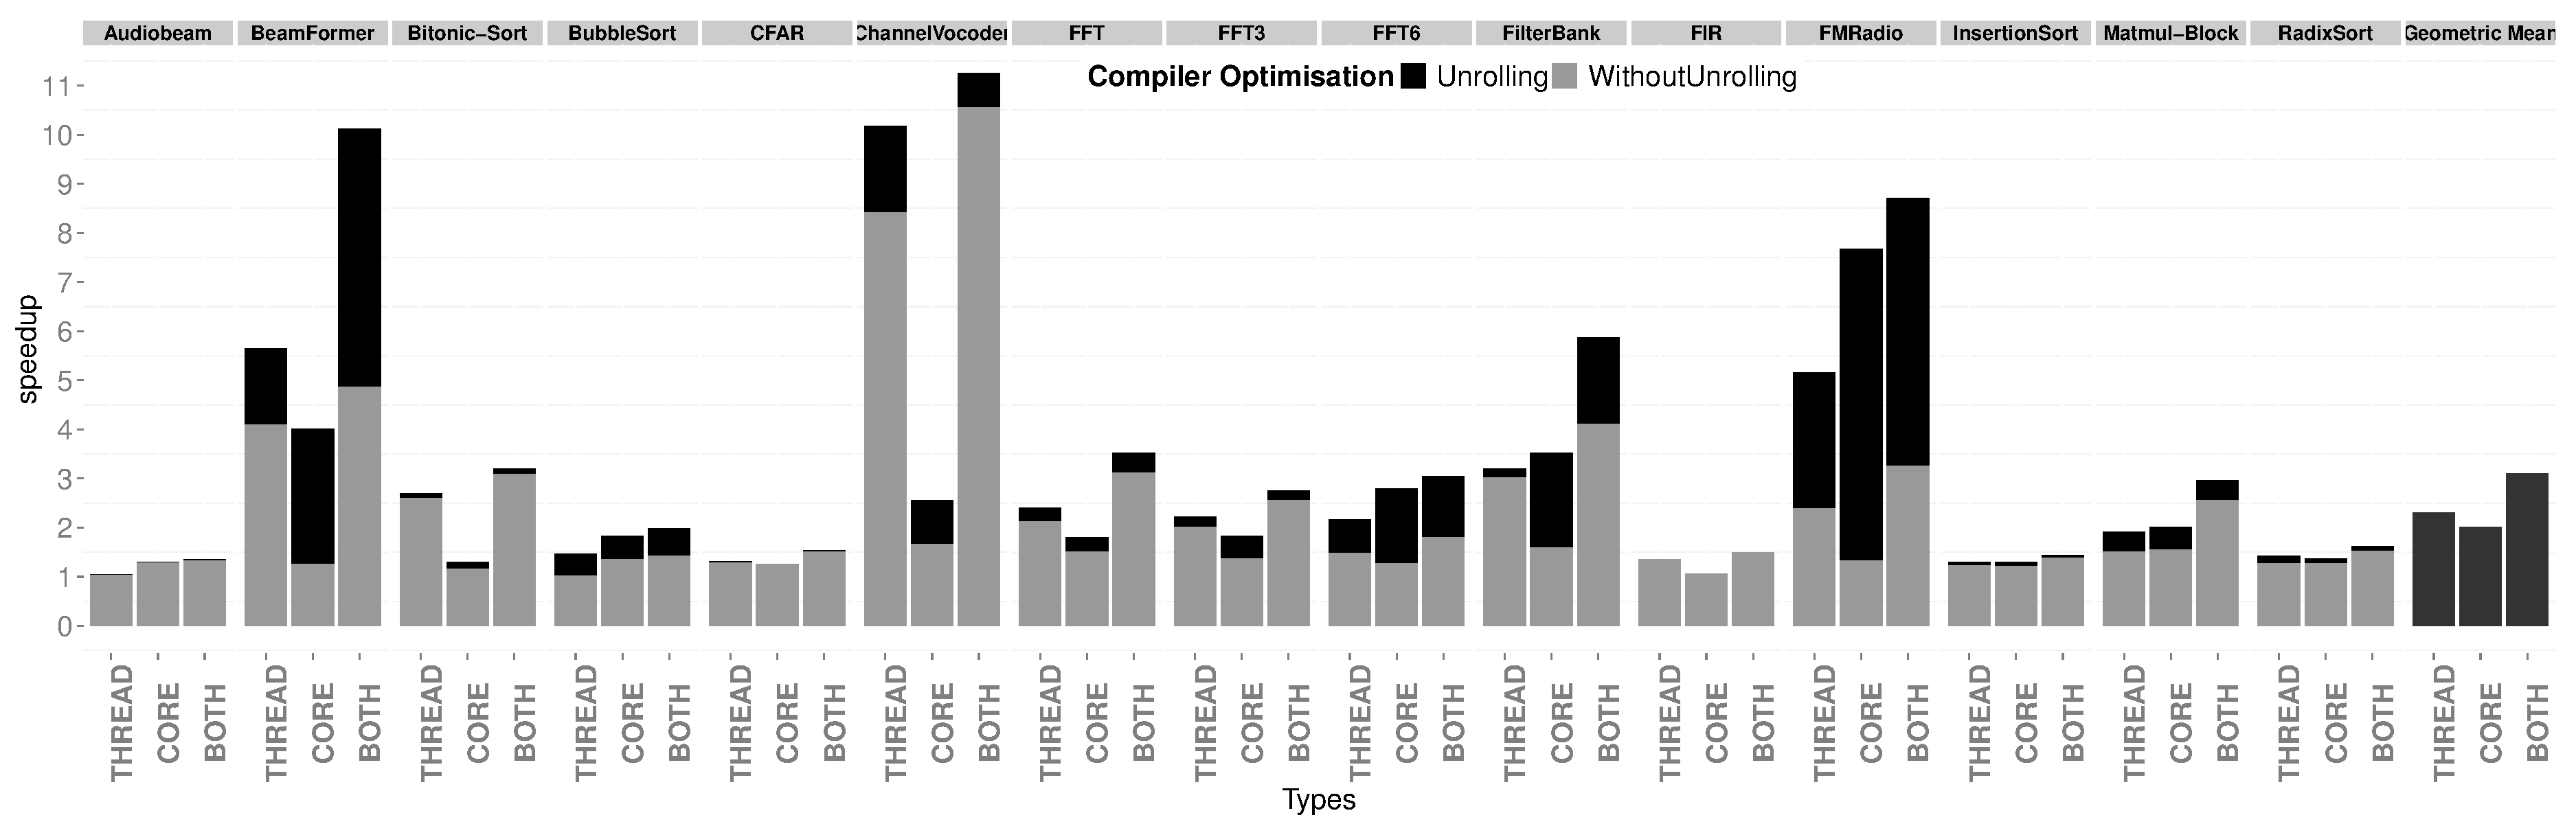
\includegraphics[width=1\linewidth,keepaspectratio]{streamit-paper/graphics/threadcompbench.pdf}
    \caption{Speedup obtained by choosing best core composition, best
      thread number and the combination of both optimisations. The baseline for the speedup measurement is single core, single thread execution using O2 compiler optimisations. Higher
      is better.}\label{fig:overviewhist}
\end{figure}
\end{landscape}
\subsection{Summary}
This section demonstrated that each parameter has a large effect on the performance of the workload.
Regardless of using core composition or not, there exists for each benchmark an optimal number of threads.
Unrolling is effective at exposing more opportunities for composition due to increased block sizes but there is a balance to strike between extracting large blocks and TLP.
Figure~\ref{fig:overviewhist} shows there is a 3x benefit (overall) by automating the partitioning of both the software (threads) and hardware (cores).



%\section{Machine Learning Models}
\label{sec:ml}
\section{Predicting the Best Number of Threads}
% Small intro, re-explain that finding thread/core pairing is complicated and thus ML is a good idea.
As seen in the previous section, selecting the right number of threads and a good combination of cores is difficult.
This difficulty arises from trying to balance between exploiting larger composed cores with block speculation and ILP and between exploiting a larger number of logical cores via TLP.

The problem can be decomposed into two stages; first, determining the right number of threads and then selecting a good core composition.
In this section, two machine-learning models that predict the best thread partitioning and core composition to maximize performance are presented.

\subsection{Synthetic Benchmark Generation}

One of the difficulties of building a machine learning based model for StreamIt is the lack of benchmarks available~\cite{wang2013partitionstreamit}.
Whilst there exists at least 30 realistic applications for StreamIt~\cite{theis2010empericalcharstreamit} this is simply not enough to create a large enough data set.
To overcome this problem generating synthetic benchmarks can be a solution~\cite{cumminsopencl2017}.
Thus synthetic StreamIt benchmarks are generated and statistics are gathered from them in a similar style as in~\cite{wang2013partitionstreamit}.
To ensure that the synthetic benchmarks are representative of realistic benchmarks they are created using filters from a set of micro-kernels found in some StreamIt applications.
30 different possible filters with different incoming and outgoing rates and different inputs and outputs types are used to increase the variety of the dataset.
To ensure that the synthetic benchmarks were similar to real benchmarks, the total number of filters and split joins are within the average of the realistic benchmarks.

For each generated application, 15 different threaded versions are generated.
Each of these versions is ran using a single core per thread and the cycle count is recorded.
This was repeated for 1000 unique randomly generated applications and record the best number of threads each time.

Once the benchmarks have been generated, the next step consists of gathering features for each applications.
In order to build the two machine learning models an initial set of over 50 features are extracted from StreamIt programs.
These features were extracted using pre-existing analytical tools within StreamIt and some counters added specifically for this chapter.
As 50 features may not necessarily contain any valuable information, the features selected for the models were determine through correlation analysis.
%In this section, when discussing correlation we specifically look at which variables correlate with the optimal number of threads.

\subsection{KNN Model}
In this section, variables which correlate with the optimal number of threads are explored.
These features are used by the model to make a prediction about the number of threads to use.
Figure~\ref{fig:corr} shows the 10 variables that correlate the most with determining the optimal thread number.
In StreamIt the term multiplicity references the number of times a filter will have to execute in a time slice when the graph is in a steady state~\cite{gordon2002streamcomp}.

\begin{figure}
  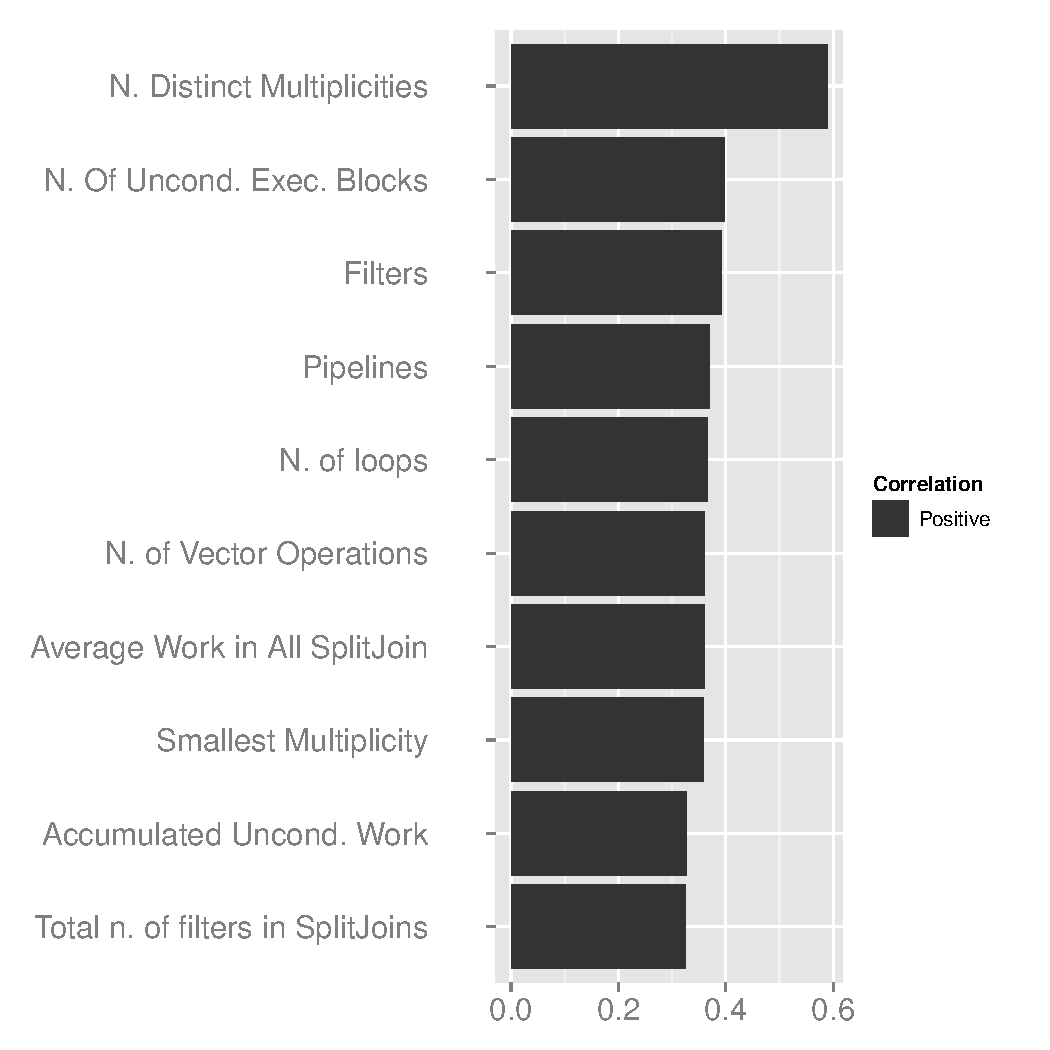
\includegraphics[width=1\textwidth]{streamit-paper/graphics/corrGraph.pdf}
  \caption{The ten highest correlating features with the best number of threads for 1000 synthetic benchmarks.}\label{fig:corr}
\end{figure}
 
\vspace{5em}
The 10 features can be described as followed:
\begin{itemize}
\item Number of Distinct Multiplicities: the variety of different execution rates of filters per time slice.
\item Number of unconditionally executed blocks: amount of operations in a filter that always execute.
\item Filters: number of filters found in the benchmark.
\item Pipelines: number of pipelines found in the benchmark.
\item Number of Loops: amount of loops present in the benchmark.
\item Number of Vector Operations: amount of potential vector operations found in the benchmark.
\item Average Work in all SplitJoins: average amount of operations per SplitJoin.
\item Smallest Multiplicity: The smallest execution rate of a single filter.
\item Accumulated Unconditional Work: Total number of operations in all filters which must be executed.
\item Total Number of filters in SplitJoins: Amount of filters that are found in SplitJoins.
\end{itemize}

According to Figure~\ref{fig:corr} the highest correlating value is Number of Distinct Multiplicitie found in the StreamIt application.
There are very little variables that highly correlate beyond Number of Distinct Multiplicities.
A high number of distinct multiplicities implies that the StreamIt application features an important amount of filters with different execution rates.
This means that certain filters may be local bottlenecks in a Pipeline for example.
When the number of distinct multiplicities is high this requires more threads to group filters with similar multiplicities together.
For example, the benchmark \bench{ChannelVocoder} only has 66\% of its filters sharing the same average multiplicity~\cite{theis2010empericalcharstreamit} of 50, with a minimum multiplicity of 1. 
The benchmark features a single SplitJoin yet when recalling section \ref{sec:streamit:dse}'s Figure~\ref{fig:overviewhist} \bench{ChannelVocoder}'s performance is greatly improved via multi-threading.
The number of threads also depends on certain structural features such as Pipelines, SplitJoins and number of Filters.
Yet, these variables seem to hold less influence on the number of threads a program needs than the different multiplicities found in the graph.
This is most certainly due to the fact that whilst SplitJoins make parallelizable areas more visible, the amount of work contained in each stream of the SplitJoin, especially when this size is small, may actually make parallelizing the program worse due to ratio of communication to computation.
It is also important to understand that a high number of Pipelines implies the use of SplitJoins.
This is due to the fact that a StreamIt application with no SplitJoins will feature only a singe Pipeline, thus a larger number of pipelines implies at least one SplitJoin.\\

A k-Nearest Neighbor (kNN) model is deployed to determine the number of threads to use for an application.
Given a new application, the kNN classifier determines the $k$ closest generated applications.
The distance between the features is measured using the Euclidean for each application.
Once the set of $k$ nearest neighbors is identified, the model simply averages the best number of threads for each of the $k$ nearest neighbors to make a prediction.
The parameter $k$ was determined experimentally using only the generated benchmarks.
A value of $k=7$ was found to lead to the best performance.
The features chosen are the ten variables displayed in Figure~\ref{fig:corr}.

Cross validation is used to determine the efficiency of the model by observing how close a classification is to the measured best thread number.
Using cross validation the model generated in this chapter has a 33\% accuracy of getting the exact best thread number.
The accuracy increases to 57\% when allowing a prediction to be 1 thread away from the best and 67\% when 2 threads away.
On average, having a thread number that is +/- 1 away from the optimal thread count only incurrs a 12\% performance penalty.
For a distance of +/- 2 this increases to 19\%.
This penalty was measured by comparing the performances of the synethtic benchmarks using only multithreading.



\section{Predicting Core Composition}
\subsection{Predicting the size of a core composition}
In Section~\ref{sec:streamit:dse}, Figure~\ref{fig:threadtrend} showed the performance of each of the 15 benchmarks when partitioning them into threads with and without core-composition.
In both cases, the number of threads is often similar.
The section also demonstrated that loop unrolling can improve the performance of core composition.

Since core composition is used to improve the performance of a single-working-thread, it is important to take into consideration that partitioning the software into threads facilitates the core estimation per thread.
Without determining a number of threads before predicting the number of cores the core-composition model has no information as to the number of threads or the structure of each thread.
In this situation, the core-composition model would either have to make its own estimates as to the thread count, or make a general prediction for a single-working-thread.
Therefore predicting core-composition comes after predicting the number of threads.

\subsubsection{Gathering Training Data for Core-Composition}
For this section the single-working-threaded version of the StreamIt benchmark are used to determine the optimal number of cores in order to explore all possible core composition sizes.
Some of the multi-threaded versions of benchmarks can be used to add extra data-points to build the model, however not all thread-counts are suitable.
One of the difficulties of adding data-points from the highly threaded versions of an applications is that each thread will only be able to have a very small core-composition.
For example, if the 15 threaded version of a benchmarks is added as data points to the model, then each of the feature vectors for this version would have a single core attributed to it.
This is due to the fact that in the 15 threaded versions of benchmarks each thread can only have a single core due to the number of cores on the DMP.
Yet, these threads could potentially benefit from core-composition, so adding them as data points to the model skews future predictions as the feature vector for each thread would associate the features to use only a single core.
Thus high-threaded versions of applications must be ignored to avoid having incorrect suggestions for core-composition sizes.

For the exploration of core composition, the 15 StreamIt benchmarks explored throughout the design space exploration are used. %explain why.
To increase the amount of data available, multiple versions of the benchmarks using different amounts of unrolling are included in the search space.
Four different levels of unrolling are used in to build the model: 0,4,16 and 64.
To determine the optimal number of cores only the training data that has a performance within 1\% of the best is selected.

\begin{figure}[t]
\centering
  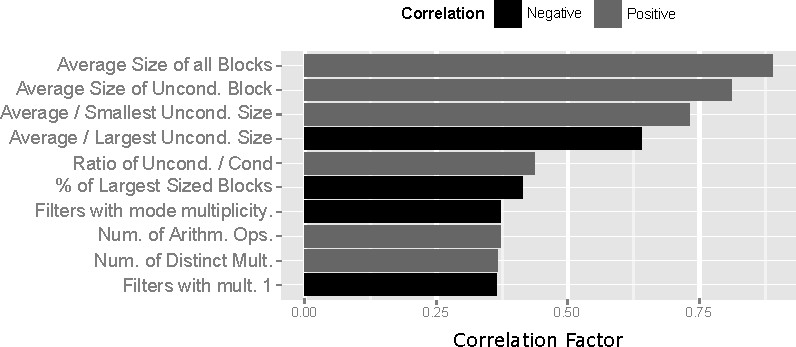
\includegraphics[width=1\textwidth]{streamit-paper/graphics/corrGraph_remix2.pdf}
  \caption{The ten highest correlating features with the optimal number of cores.}\label{fig:corrCore}
\end{figure}


\subsubsection{Correlation Analysis}

Figure~\ref{fig:corrCore} shows the highest correlating features with the optimal number of cores.

The ten features can be described as follows
\begin{itemize}
\item Average Size of All Blocks: Average number of operations per block of code.
\vspace{-1em}
\item Average Size of Unconditional Blocks: Average number of operations per blocks that must execute unconditionally.
\vspace{-1em}
\item Average / Smallest Unconditional Size: The ratio between the average size of a block compared to the smallest size of unconditional blocks.
\vspace{-1em}
\item Average / Largest Unconditional Size: The ratio between the average size of a block compared to the largest size of unconditional blocks.
\vspace{-1em}
\item Ratio of Unconditional Blocks to Conditional Blocks.
\vspace{-1em}
\item Percentage of blocks that have the largest number of operations.
\vspace{-1em}
\item Filters with mode multiplicity: number of filters that have the average mode multiplicity.
\vspace{-1em}
\item Number of arithmetic operations found in the program.
\vspace{-1em}
\item Number of distinct multiplicites found in the program.
\vspace{-1em}
\item Number of filters that have a multiplicity of 1.
\end{itemize}


The features are very different from the ones presented in Figure~\ref{fig:corr} and overall there are features which correlate higher with core-compositions than number of threads.
The highest correlating value, which is the average size of a block, has a correlation factor of 0.88.
It is important to note that the concept of an operation here is at the StreamIt level and not the architectural level.
This is because the machine learning model will get information from the source-level StreamIt translation.
With that in mind, the number of operations will correlate with the number of instructions found at the instruction level.

The second feature is similar to the first but only takes into account blocks that will be executed unconditionally.
Blocks found in loops are excluded for this metric as there is still some form of condition for those blocks to be executed.
The next two features compare the average size of an unconditional block to the largest and smallest unconditional block.
The fifth feature measures the ratio of the number of unconditional blocks to conditional.

Overall the highest correlating features are not features distinct to StreamIt, such as Pipelines or SplitJoins.
This is due to the fact that, from a single-threaded perspective, SplitJoins and Pipelines are less visible in terms of performance.
This is especially true of SplitJoins as they will not be distributing data amongst different threads and, technically, a single-threaded StreamIt program is a long pipeline structure.
It can thus be inferred that the optimal number of cores is independent of the structure of a StreamIt program.
Instead determining the correct core-composition is more dependent on the amount of computation found in each program.

From Figure~\ref{fig:corrCore} the highest correlating features fit naturally under the assumptions that higher core compositions will perform better with larger blocks of operations and thus blocks of instructions.
When blocks are small, a single core can fetch and execute multiple blocks in parallel; up to 4 blocks per core when blocks are smaller than 32 instructions.
Cores in a composition do not fetch blocks independently; instead one of the cores in the composition will start by fetching blocks until all its lanes are used and then submits the following predicted PC to the next core in the composition.
If blocks are small this means that core-compositions will have to predict a high number of blocks to fill up all its cores.
Thus large blocks reduce the number of predictions required to populate all the cores with blocks, reducing the latency of fetching blocks for all cores.
The necessity to correctly predict blocks to ensure that all cores are fully utilised explains why a higher number of unconditionally executed blocks compared to conditional blocks correlates positively with large core compositions.

The importance of size is also apparent as the difference between the largest block size and the average block size negatively correlates with core-composition.
The ratio of unconditional and conditional blocks is considered less important than block size due to branch prediction, however having a larger number of unconditional branches is a natural fit for larger core-compositions as it reduces the dependency on high branch-prediction accuracy.

Other features that are analysed included more fine-grained data such as the types of operations that are found in the blocks of code.
This involved finding ratios of floating point, integer and memory operations.
However, according to the correlation graph in Figure~\ref{fig:corrCore}, the constitution of these blocks of code is not as important as their size or whether they are conditionally executed.

\begin{figure}[t]
  \center
  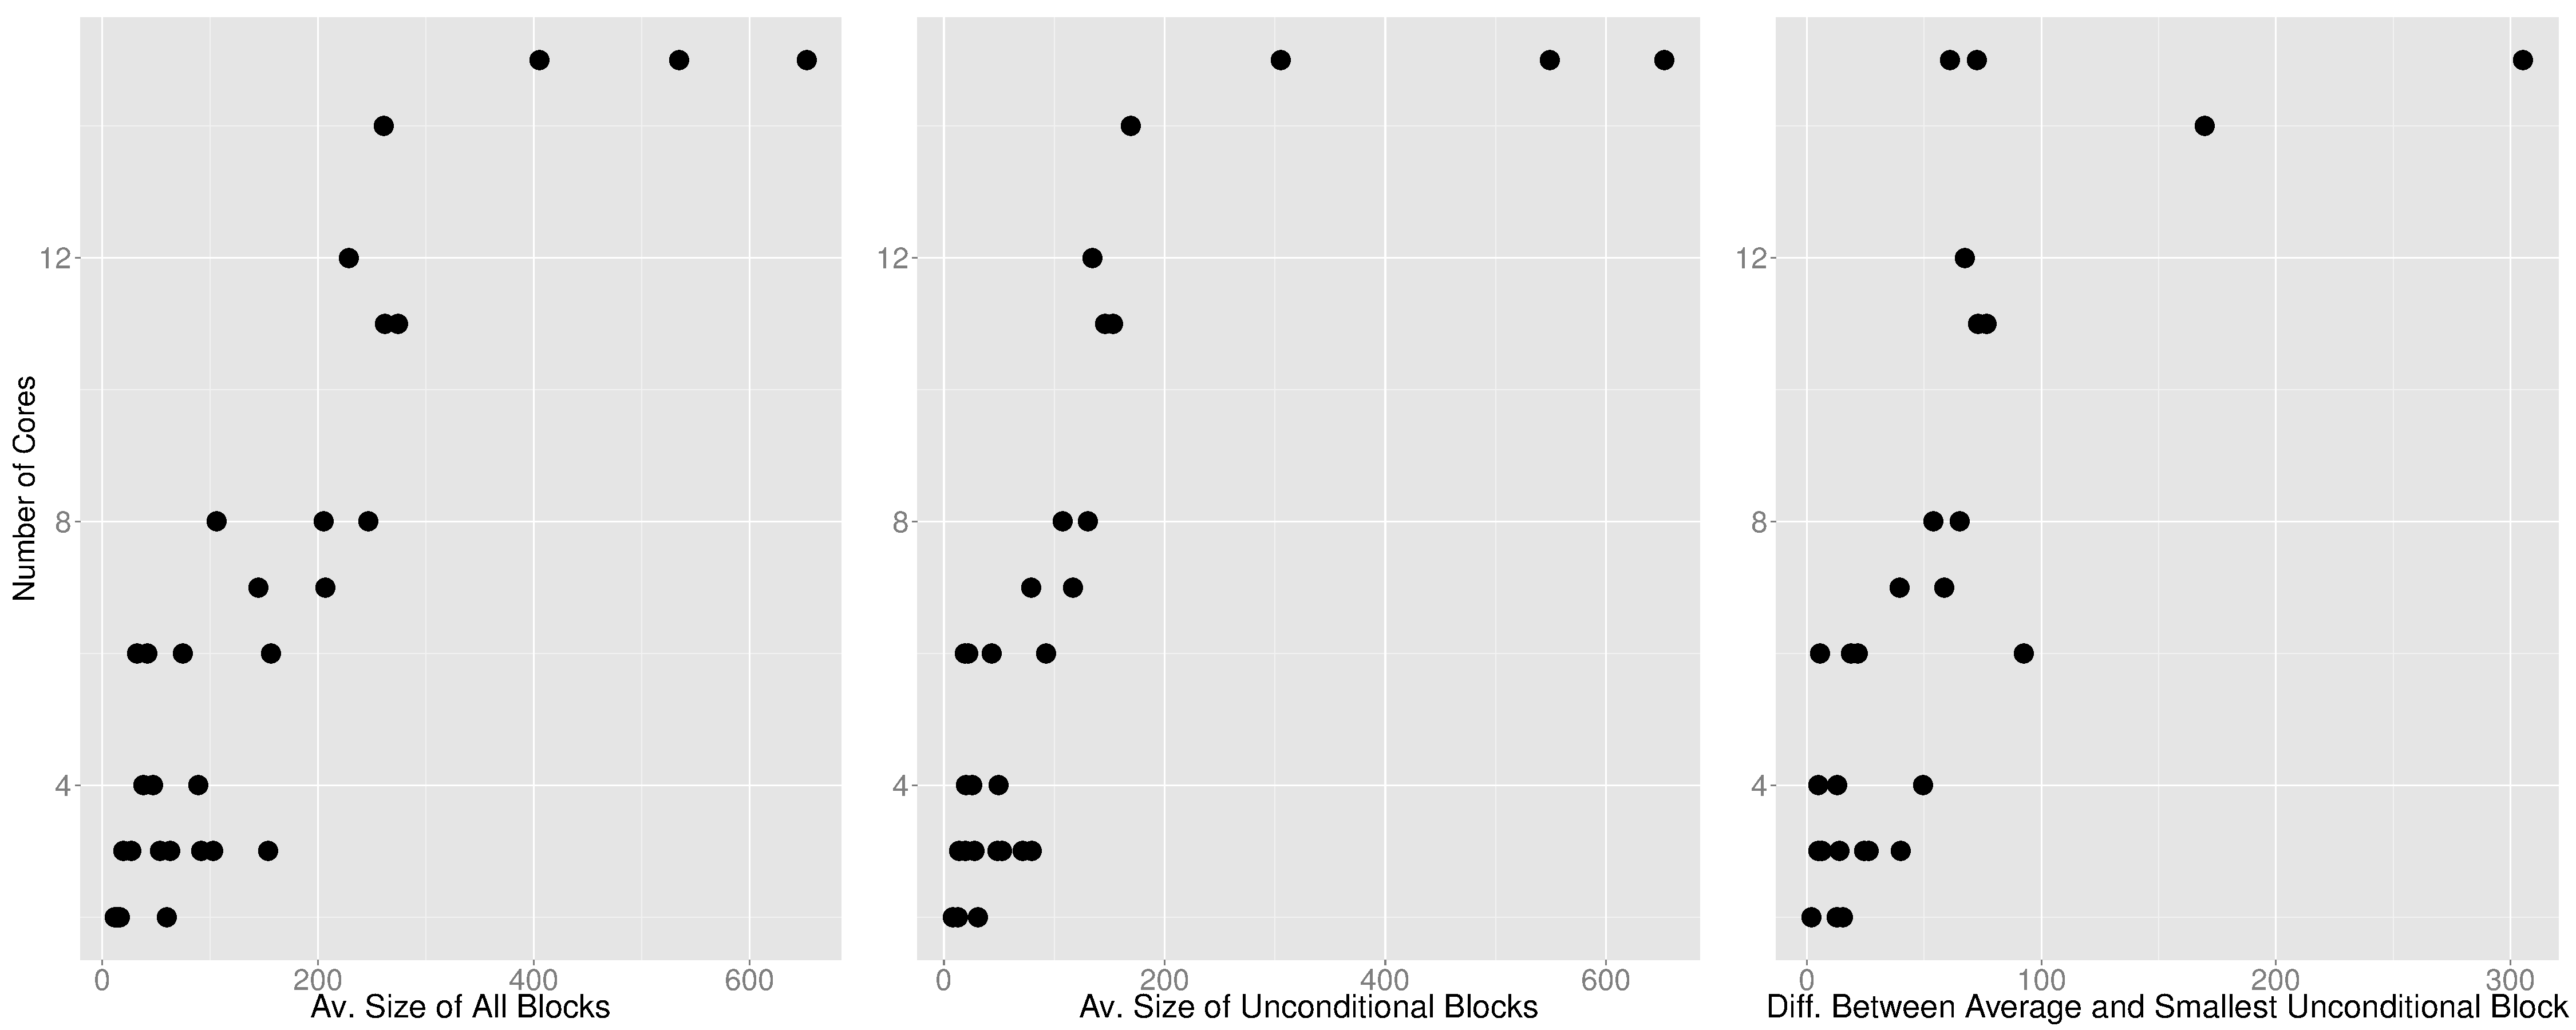
\includegraphics[width=1\textwidth]{streamit-paper/graphics/lineargraphs.pdf}
  \caption{Optimal number of cores in relation to the three highest correlating features. The maximum number of cores plateaus on the right hand side as this is the maximum possible amount.}\label{fig:maxav}
\end{figure}

\subsubsection{Linear Regression Model}
Given that the optimal number of cores highly correlates with a few features, a linear regression is a natural choice to predict the best number of threads.
Figures~\ref{fig:maxav} represent how the first three highest correlating values affect the optimal number of cores for a single-working-thread.
This figure is obtained by finding the best number of cores for the single-working-threaded version of each of the StreamIt benchmarks whilst varying the amount of loop unrolling.
It is important to note that the reason the points in the top right corner appear to converge at 15 cores is due to the fact that no more than 15 cores can be fused.
Overall, Figure~\ref{fig:maxav} shows that StreamIt applications with large unconditionally executed blocks will require large compositions.




%\section{Compiler Optimisation}
%\begin{figure}[t]
\begin{minipage}[t]{0.48\textwidth}
\lstset{language=C,numbersep=4pt,basicstyle=\small}
\begin{lstlisting}
for(int i = 0; i < 1000; i++)
  for(int j = 0; j < 1000; j++)
     for(int k = 0;k < 5; k++)
         a[i][j] = a[i][j] * b[k][j];
\end{lstlisting}
\vspace*{-5mm}
\caption{Example of an inner-most loop which should be completely unrolled.}
\label{lst:small}
\end{minipage}
\hfill
\begin{minipage}[t]{0.48\textwidth}
\lstset{language=C,numbersep=4pt,basicstyle=\small}
\begin{lstlisting}
for(int i = 0; i < 1000; i++)
  for(int j = 0; j < 1000; j++)
      a[i][j] = a[i][j-1] 
                       * b[i][j];
\end{lstlisting}
\vspace*{-5mm}
\caption{Example of a data dependency which can be removed by interchanging the loops.}
\label{lst:dep}
\end{minipage}
\vspace{9mm}
\end{figure}

This section describes optimizations focused on reducing control flow and expanding block sizes which is necessary for high performance as seen in section~\ref{sec:lim_study}.

\subsection{Loop Unrolling}
Loop unrolling is a common optimization used to reduce the overhead of the loop header and to better expose Instruction Level Parallelism (ILP).
When dealing with tightly-knit loops, logical cores may perform poorly due to the fact that they execute many small blocks, thus increasing the Synchronization Cost.
Unrolling loops will both reduce the number of blocks required to execute the loop and increase the size of the blocks, thus reducing the Synchronization Cost and increasing ILP.
For example, the innermost loop in Figure~\ref{lst:small} should be completely unrolled and its outer loop unrolled partially to increase the block size.
There are certain factors which can limit the usefulness of loop unrolling which we examine later on.
In the architecture we evaluate, we may not have more than 32 load or store instructions per block.
Therefore, if we unroll memory intensive loops, we must ensure we do not go above this threshold.
Going above this threshold leads to creating a new block which will put a strain on the branch predictor.
Another issue is that unrolling loops with conditional statements may not help improve the size of the block as the conditional branches might still segment the new blocks.
So we should avoid unrolling such loops.



\subsection{Loop Interchange}
When dealing with nested loops there is one reason we have determined for interchanging the loops.
The case arises when interchanging the loop removes dependencies in the inner-most loop.
The dependency in Figure~\ref{lst:dep} can be removed by interchanging the loops. 
This allows us to unroll the inner loop efficiently, but also remove any kind of dependency between blocks.
Since two blocks from the same loop may execute on different cores, we want to reduce any kind of data dependency, minimizing core communication.

\begin{figure}[t]
     \centering
     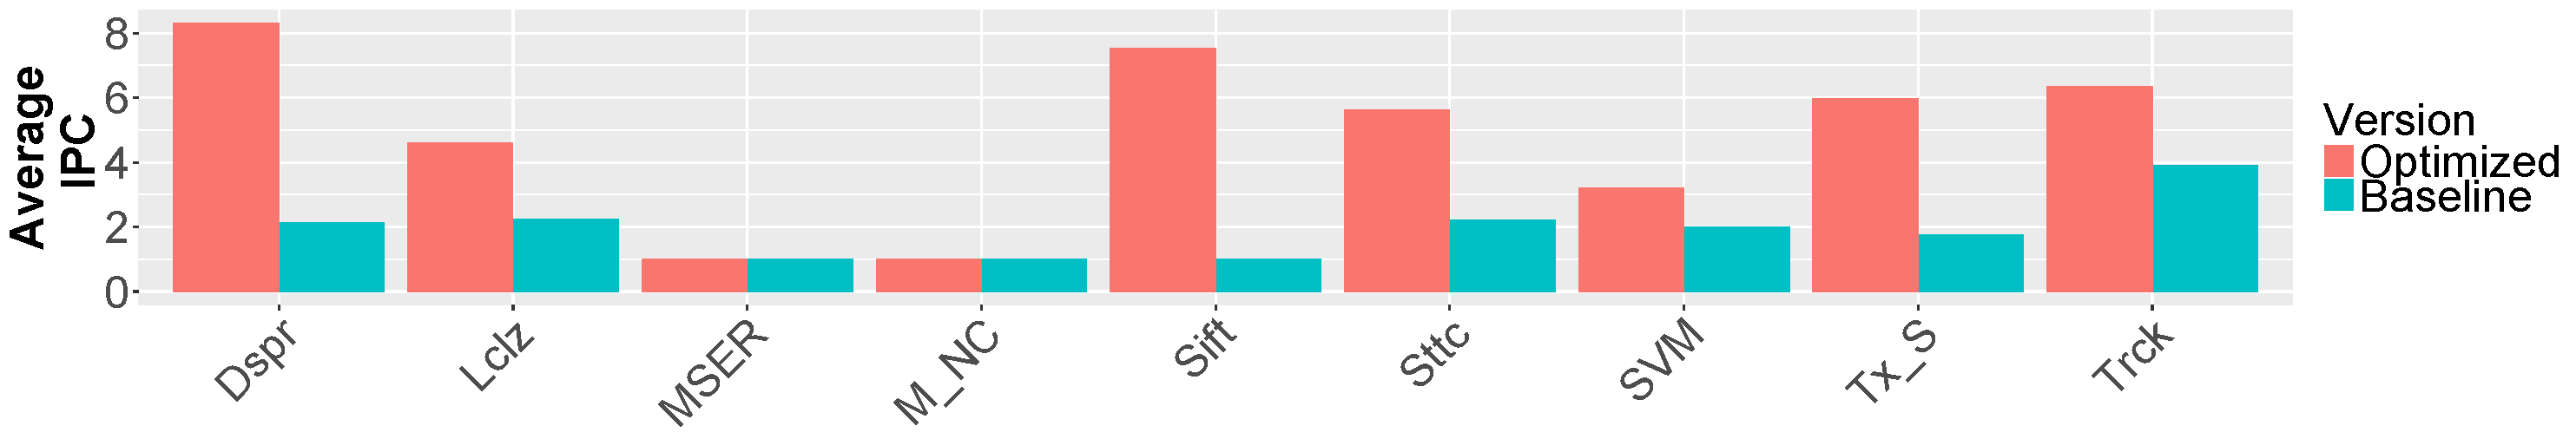
\includegraphics[width=\textwidth]{graphics/Exploration/ipc_comp.pdf}
\vspace*{-8mm}
     \caption{Average IPC using the optimal sized logical-core, with and without optimizations. Higher is better.}
     \label{fig:ipccom}
     \vspace{0.5em}
\vspace{5mm}
    \centering
    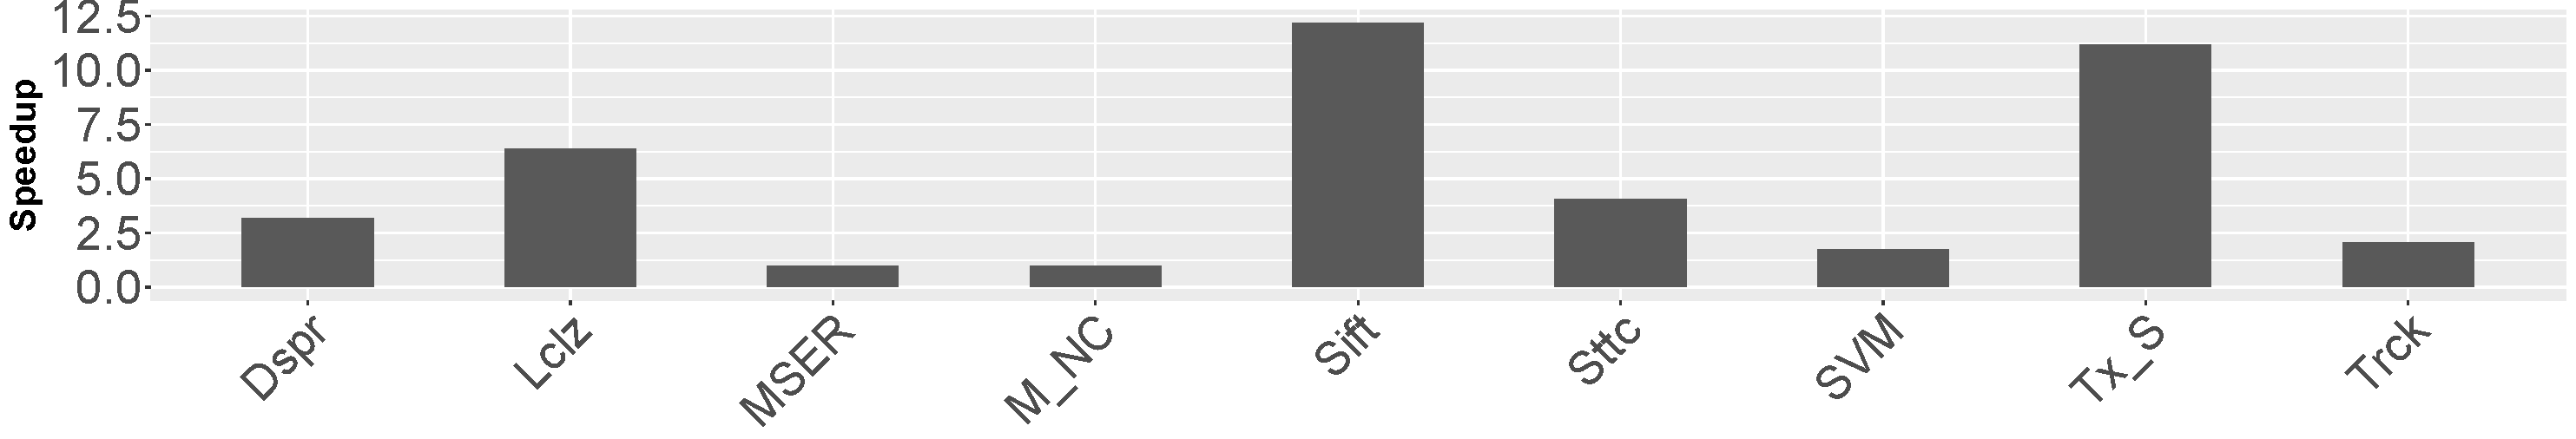
\includegraphics[width=\textwidth]{graphics/Exploration/comp_speed.pdf}
\vspace*{-8mm}
    \caption{Speedup from using code-optimizations over baseline source code using the same optimal sized logical-core.}
    \label{fig:speedcomp}
\vspace{5mm}
\end{figure}

\subsection{Predication and Hyperblock Formation}
EDGE compilers must split blocks whenever control-flow is present~\cite{smith2006edge}.
If a loop contains a conditional statement, the loop body has to be split in two unless if-conversion is applied.
Hyperblock formation aims to reduce branching and increase block size by combining two or more blocks into a single predicated block~\cite{smith2006edge}.
Hyperblocks reduce both synchronization cost and branch prediction requirements as discussed previously.
This is especially important in control-flow intensive loops where unrolling increases the number of conditional statements.

\vspace{5mm}
\subsection{Results}

While the optimizations described above and their tuning would be easy to implement in a compiler, we did not have access to the compiler's source code.
We therefore modified the source code of our benchmarks by manually interchanging or unrolling loops.
In the case of predication and hyperblock formation, we converted simple if-then-else statements into ternary operators whenever possible.
We also tried to reorder statements within the body of a loop to avoid having control flow in the middle of the body.
We then verified that our source code modification had the intended effect by dissembling the binary produced by the compiler.
We modified between 0 and 12 loops depending on the benchmark.

We compare the best static core fusion using the optimized code with the unmodified code, both version compiled with \texttt{-O2}.
Figure~\ref{fig:ipccom} shows the resulting IPC for the baseline case and the optimized benchmarks when run on a core with the optimal number of fused core to maximize performance.
The IPC of the baseline is very low for the majority of the benchmarks which might give the impression that core fusion is rather inefficient.
However, after applying the simple optimizations described above, the average IPC is significantly increased in many cases.

Since optimizations change the total number of instructions, we also show the actual speedup obtained using cycle count in Figure~\ref{fig:speedcomp}.
As we can see, benchmarks \bm{MSER} and \bm{Multi-NCut} do not perform any differently.
This is due to the fact that none of these optimizations can be successfully applied on these benchmarks.
For the other benchmarks we see significant improvements of up to 12$\times$ for \bm{Sift} when the optimizations are applied.

\subsection{Summary}

Overall, this section shows that classical loop transformations can have a large impact on the performance of fused cores.
Without these optimizations, it would be more difficult to motivate the use of core fusion even at a static-level as the IPC does not deviate enough from a single core.


\section{Results}
\label{sec:results}
This section describes the performance achieved by the model when predicting the number of threads and core composition to use for each of the StreamIt benchmarks and compares it to the optimal solution found when exploring the space.

\begin{figure}[t]
    \centering
    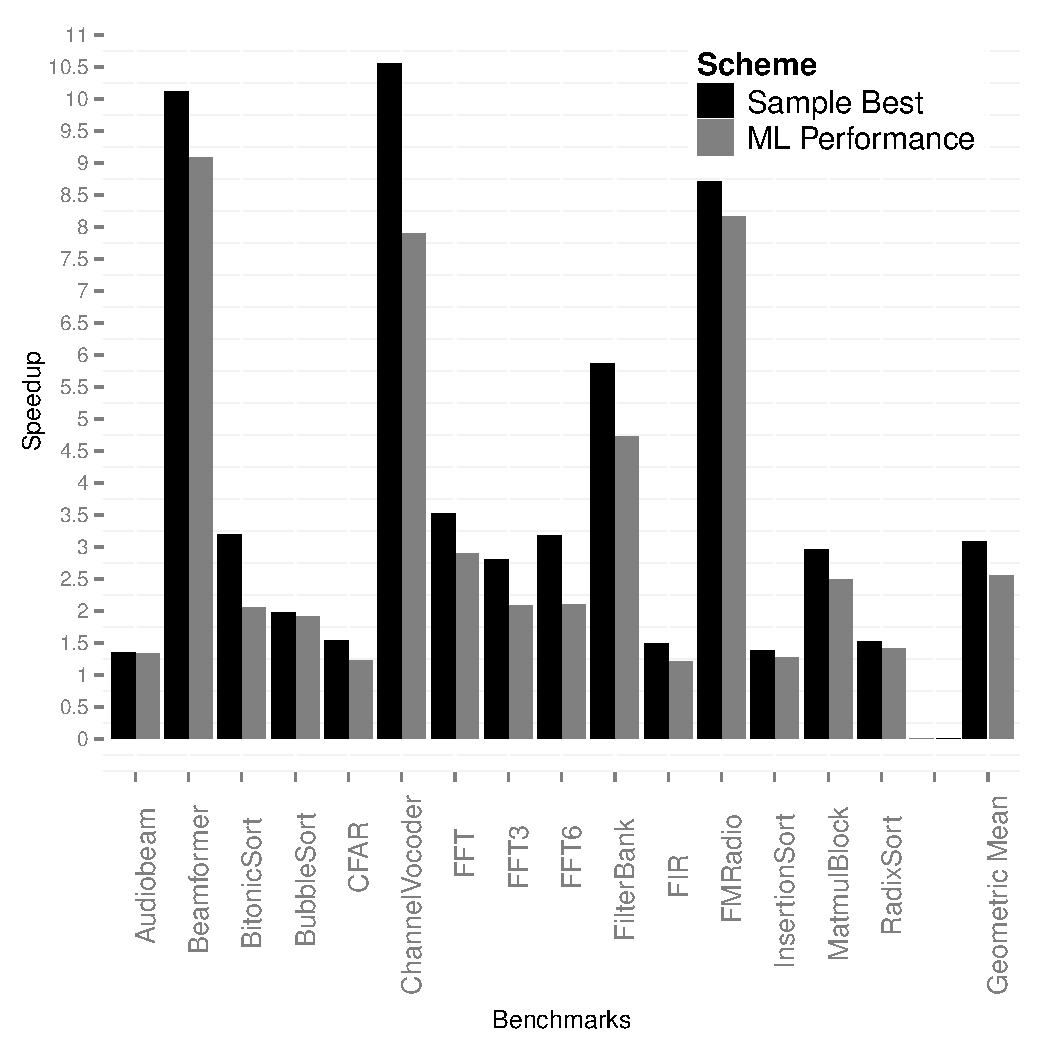
\includegraphics[width=0.7\textwidth]{streamit-paper/graphics/results.pdf}
    \caption{Performance of the machine learning model against the best execution from random sampling. The baseline for the speedup measurement is single core, single thread execution using O2 compiler optimisations. Higher is better.}\label{fig:results}
\end{figure}

\subsection{Machine Learning Model Evaluation Methodology}

Leave-one-out cross-validation is used for testing the linear model.
This means that when testing the model on one application, this application is removed from the training set, the model is trained with the remaining application and finally the model is tested on the application; this process is repeated for each application.
This is standard methodology in the machine-learning community ensuring that the training data is never used for testing.
For the kNN model, the training data consists of all the generated synthetic benchmarks and it is only tested on the real StreamIt applications as they are not used for training.
To obtain the speedup the performance of the machine learning based result are compared to the best from the sample space to running the StreamIt benchmark on a single core, single thread, using O2 compiler optimisations. 

\subsection{Evaluation}

Figure~\ref{fig:results} compares the performance of the machine-learning model and the best performance from the sample space.
As explained in the earlier section, the sampled best is drawn from a sample size of 1,316 combinations of core compositions and thread partitions for each application when possible.
The baseline is the original StreamIt application running with one thread and one core with O2 optimisations on the dynamic multicore processor.
The average speedup obtained through the machine learning model is 2.6 compared to the baseline, this is only 16\% smaller than the average of the best found, which is a speedup of 3.1.
These results are positive as it means the model's results are at least within 16\% of the total best.

As can been seen in Figure~\ref{fig:results} the largest performance penalty resides in the performance of \bench{ChannelVocoder}.
Table~\ref{tab:summary} presents the actual configuration found for the best sampled point and the machine learning model prediction.
Each column represent a different threads and the number in the cell represents the number of core associated with that thread.
For ~\bench{ChannelVocoder} the model predicts only 8 threads rather than the optimal 13.
Referring back to Figure~\ref{fig:threadtrend} and Figure~\ref{fig:overviewhist} from Section~\ref{sec:streamit:dse} \bench{ChannelVocoder} always performs better when adding more threads rather than increasing the size of a core composition.
This is the cause of the performance penalty, for ~\bench{ChannelVocoder} it is more important to allocate a higher number of threads rather than compose cores.
Aside from this case, the machine learning model obtains similar speedups to the best sample.

\begin{table*}[t]
\centering
\resizebox{0.75\textwidth}{!}{\begin{minipage}{0.5\textwidth}
  \small
  \hspace{-5em}
 \begin{tabular} { | l | l | l | l | l | l | l | l | l | l |l| }
    \hline
      & \textbf{1} & \textbf{2} & \textbf{3} & \textbf{4} & \textbf{5} & \textbf{6} & \textbf{7} & \textbf{8} & \textbf{9} & \textbf{10} \\ \hline
    B Audiobeam & 3 & 2 & \cellcolor[gray]{0.3}& \cellcolor[gray]{0.3}& \cellcolor[gray]{0.3}& \cellcolor[gray]{0.3}& \cellcolor[gray]{0.3}& \cellcolor[gray]{0.3}& \cellcolor[gray]{0.3}& \cellcolor[gray]{0.3} \\ \hline 
    M Audiobeam & 2 & 3 & \cellcolor[gray]{0.3}& \cellcolor[gray]{0.3}& \cellcolor[gray]{0.3} & \cellcolor[gray]{0.3}& \cellcolor[gray]{0.3}& \cellcolor[gray]{0.3}& \cellcolor[gray]{0.3}& \cellcolor[gray]{0.3}\\ \hline\hline
    B Beamformer & 1 & 4 & 2 & 4 & 4& \cellcolor[gray]{0.3}& \cellcolor[gray]{0.3}& \cellcolor[gray]{0.3}& \cellcolor[gray]{0.3}& \cellcolor[gray]{0.3} \\ \hline 
    M Beamformer & 6 & 4 & 4& \cellcolor[gray]{0.3}& \cellcolor[gray]{0.3}& \cellcolor[gray]{0.3}& \cellcolor[gray]{0.3}& \cellcolor[gray]{0.3}& \cellcolor[gray]{0.3}& \cellcolor[gray]{0.3} \\ \hline\hline
    B BitonicSort & 3 & 2 & 2 & 2 & \cellcolor[gray]{0.3}& \cellcolor[gray]{0.3}& \cellcolor[gray]{0.3}& \cellcolor[gray]{0.3}& \cellcolor[gray]{0.3}& \cellcolor[gray]{0.3}  \\ \hline
    M BitonicSort & 1 & 2 & 2 & 1 & 2 & 2 & 2 & \cellcolor[gray]{0.3}& \cellcolor[gray]{0.3}& \cellcolor[gray]{0.3} \\ \hline\hline
    B BubbleSort & 3 & 3& \cellcolor[gray]{0.3} & \cellcolor[gray]{0.3} & \cellcolor[gray]{0.3}& \cellcolor[gray]{0.3}& \cellcolor[gray]{0.3}& \cellcolor[gray]{0.3}& \cellcolor[gray]{0.3}& \cellcolor[gray]{0.3} \\ \hline
    M BubbleSort & 2 & \cellcolor[gray]{0.3} & \cellcolor[gray]{0.3} & \cellcolor[gray]{0.3} & \cellcolor[gray]{0.3}& \cellcolor[gray]{0.3}& \cellcolor[gray]{0.3}& \cellcolor[gray]{0.3}& \cellcolor[gray]{0.3}& \cellcolor[gray]{0.3} \\ \hline\hline
    B CFAR & 3 & 2 & \cellcolor[gray]{0.3} & \cellcolor[gray]{0.3} & \cellcolor[gray]{0.3}& \cellcolor[gray]{0.3}& \cellcolor[gray]{0.3}& \cellcolor[gray]{0.3}& \cellcolor[gray]{0.3}& \cellcolor[gray]{0.3} \\ \hline 
    M CFAR & 2 & 2  & 1  & 2 & \cellcolor[gray]{0.3}& \cellcolor[gray]{0.3}& \cellcolor[gray]{0.3}& \cellcolor[gray]{0.3}& \cellcolor[gray]{0.3}& \cellcolor[gray]{0.3} \\ \hline\hline
    B ChannelVoc.& 4 & 1 & 1 & 1 & 1 & 1 & 2 & 1 & 1 & 1 \\ \hline 
    M ChannelVoc.& 2 & 2 & 1 & 2 & 2& 2 & 2& \cellcolor[gray]{0.3}& \cellcolor[gray]{0.3}& \cellcolor[gray]{0.3} \\ \hline\hline
    B FIR & 3 & 2 &\cellcolor[gray]{0.3}&\cellcolor[gray]{0.3}&\cellcolor[gray]{0.3}&\cellcolor[gray]{0.3}&\cellcolor[gray]{0.3}&\cellcolor[gray]{0.3}&\cellcolor[gray]{0.3}&\cellcolor[gray]{0.3}\\ \hline
    M FIR & 2 & 2&\cellcolor[gray]{0.3}&\cellcolor[gray]{0.3}&\cellcolor[gray]{0.3}&\cellcolor[gray]{0.3}&\cellcolor[gray]{0.3}&\cellcolor[gray]{0.3}&\cellcolor[gray]{0.3}&\cellcolor[gray]{0.3}\\ \hline\hline
    \end{tabular}
  \end{minipage}	\hfill
  \hspace{1em}
\begin{minipage}{0.5\textwidth}

	 \begin{tabular} { | l | l | l | l | l | l | l |}
    \hline
      & \textbf{1} & \textbf{2} & \textbf{3} & \textbf{4} & \textbf{5} & \textbf{6}  \\ \hline

	B FFT & 3 & 3 & 5 & \cellcolor[gray]{0.3}& \cellcolor[gray]{0.3}& \cellcolor[gray]{0.3} \\ \hline
    M FFT & 6& 5 & 2& \cellcolor[gray]{0.3}& \cellcolor[gray]{0.3}& \cellcolor[gray]{0.3}  \\ \hline\hline
    B FFT3 & 3 & 2 & 2& \cellcolor[gray]{0.3}& \cellcolor[gray]{0.3}& \cellcolor[gray]{0.3} \\ \hline 
    M FFT3 & 3 & 2 & 3 & 3& 3& 3 \\ \hline\hline
    B FFT6 & 7 & 8& \cellcolor[gray]{0.3}& \cellcolor[gray]{0.3}& \cellcolor[gray]{0.3}& \cellcolor[gray]{0.3}\\ \hline
    M FFT6& 14 & \cellcolor[gray]{0.3}& \cellcolor[gray]{0.3}& \cellcolor[gray]{0.3}& \cellcolor[gray]{0.3}& \cellcolor[gray]{0.3} \\ \hline\hline
    B FilterBank & 4 & 5 & 6& \cellcolor[gray]{0.3}& \cellcolor[gray]{0.3}& \cellcolor[gray]{0.3} \\ \hline
    M FilterBank & 4 & 5 & \cellcolor[gray]{0.3} & \cellcolor[gray]{0.3}& \cellcolor[gray]{0.3}& \cellcolor[gray]{0.3}\\ \hline\hline
    B FMRadio & 7 & 6 & \cellcolor[gray]{0.3}& \cellcolor[gray]{0.3}& \cellcolor[gray]{0.3}& \cellcolor[gray]{0.3}\\ \hline
    M FMRadio & 7 & 4 & \cellcolor[gray]{0.3} & \cellcolor[gray]{0.3}& \cellcolor[gray]{0.3}& \cellcolor[gray]{0.3} \\ \hline\hline
    B InsertionSort & 3 & 2& \cellcolor[gray]{0.3}& \cellcolor[gray]{0.3}& \cellcolor[gray]{0.3}& \cellcolor[gray]{0.3} \\ \hline
    M InsertionSort & 3 & \cellcolor[gray]{0.3}& \cellcolor[gray]{0.3}& \cellcolor[gray]{0.3}& \cellcolor[gray]{0.3}& \cellcolor[gray]{0.3}\\ \hline\hline
    B MatmulBlock & 3 & 4 & 6 & 2 & \cellcolor[gray]{0.3} & \cellcolor[gray]{0.3}\\ \hline
    M MatmulBlock & 4 & 4 & \cellcolor[gray]{0.3}& \cellcolor[gray]{0.3}& \cellcolor[gray]{0.3}& \cellcolor[gray]{0.3}\\ \hline\hline
    B RadixSort & 3 & 3& \cellcolor[gray]{0.3}& \cellcolor[gray]{0.3}& \cellcolor[gray]{0.3}& \cellcolor[gray]{0.3}\\ \hline
    M RadixSort & 2 & 2& \cellcolor[gray]{0.3}& \cellcolor[gray]{0.3}& \cellcolor[gray]{0.3}& \cellcolor[gray]{0.3}\\ \hline
    
 \end{tabular}
  \end{minipage}}
  \caption{Number of Threads and Cores used for Best of Sample Space and Machine Learning Model.}\label{tab:summary}

\end{table*}

 \subsection{Summary}

This section has demonstrated that it is possible to build a machine-learning model that achieves high level of performance using simple source code static features.
In many applications, the model even comes very close to the best from the sampled space, showing that the features used by the model contain enough information to inform the model about the best decision.

\vspace{5mm}


%\section{Related Work}
%\label{sec:related}
%\paragraph{Dynamic Multicore Processors}

DMPs such as CoreFusion~\cite{ipek2007CoreFusion} differentiate themselves to EDGE based DMPs on their Instruction Set Architecture (ISA).
CoreFusion uses a CISC/RISC based architecture which limits the degree of scalability (fusion), whereas EDGE based DMPs have shown promising scalability~\cite{kim2007composablelight, sibi2014}.
Other types of DMPs such as WidGET~\cite{Watanabe2010Widget} and Sharing Architecture~\cite{zhou2014sharingarch} present a fine-grain level of composition.
In these two architectures, cores can be created out of different components on the processor, including ALUs, floating point units and memory units.
This differs from CoreFusion and EDGE where a logical core is composed out of a set of physical cores.
This fine-grained composition can allow for even more optimisation but it increases the complexity of the problem.

\paragraph{Core Configuration}

Little work has been done on automatically determining the correct core composition for a given application.
The work conducted in~\cite{ipek2007CoreFusion,kim2007composablelight} manually configure their processors before running benchmarks.
In~\cite{santos2013nocdmc} they use information provided by the application to determine how to reconfigure some components of the processor.
This initial information then assists the rest of the reconfiguration, this process still requires input from the programmer though.
Therefore we present a novel method for automating the choice of core composition.  

\vspace{2mm}
\paragraph{Streaming Programming Languages}

There exist streaming languages that target different architectures.
For example Brook~\cite{buck2004brook} is designed to be used on GPUs and WaveScript for embedded systems~\cite{newton2008wavescript}.
These languages present different constructs to StreamIt, in particular they lack the graph oriented constructs. 
Lacking such constructs make these languages less attractive for tiled processors.

\paragraph{Partitioning StreamIt on multicore chip}

Previous work on scheduling streaming applications onto DMPs or heterogenous multicore chips focuses on finding mathematical ways of partitioning the graph onto the chip ~\cite{carpenter2009streammap,kudlur2008orchestratingstreamprog}.  
In Carpenter et al.'s work~\cite{carpenter2009streammap} they restrain themselves to partitioning a StreamIt application maintaining connectedness.
Connectedness can be defined as a subgraph where the filters are connected. 
This restriction reduces the number of potential partitions that can be generated by their algorithm and will put TLP in favour of ILP. 
Kudlur et al. in~\cite{kudlur2008orchestratingstreamprog} choose to represent the partitioning problem as an integer linear programming problem.
They start by fissionioning stateless filters to obtain the optimal load balance across all cores and assign the filters to a core using a modulo scheduler.
Farhad et al. also use integer linear programming in~\cite{farhad2012streamilp} to schedule StreamIt programs on multicore.
They profile the communication costs of the streaming programs by running the program using different multicore allocations and feed that information into their integer linear programming model.

\paragraph{Machine Learning} Using a machine learning model to partition StreamIt programs was previously explored in the work of Wang et al. in ~\cite{wang2013partitionstreamit}.
They use a k nearest neighbor model to determine the perfect partitioning of a StreamIt program for a multicore system. 
The features we extracted using correlation analysis are similar to those presented in the work of ~\cite{wang2013partitionstreamit}.
Unlike our work their model is used to find ways of fusing and fissioning filters to discover a new graph that can then be mapped onto a multicore system.



\section{Conclusion}
\label{sec:conclusion}
In this paper we presented the problem of partitioning both software and hardware for a Dynamic Multicore Processor.
We analysed a set of streaming workloads based on StreamIt, extracting features which highly influence both the required number of threads and core composition.
Using this data we introduced a machine learning model which is able to determine how many threads a StreamIt application needs and pick an appropriate chip topology.
The model predicts configurations close to the performance of the best design points from the sampled space.
By automating the decision of core composition we motivate the use of DMPs for accelerating applications without any involvement from the programmer.


%\section*{Acknowledgements}
%\label{sec:acknowledgements}
%This work has been supported by Microsoft Research through its PhD Scholarship Programme and has made use of the resources of the Edinburgh Compute and Data Facility (ECDF)~\cite{ecdf}.


%\acks
%
%Acknowledgments, if needed.
%\balance
%\bibliographystyle{abbrvnat}
%\bibliography{references}


%                       Revision History
%                       -------- -------
%  Date         Person  Ver.    Change
%  ----         ------  ----    ------

%  2013.06.29   TU      0.1--4  comments on permission/copyright notices

